\documentclass[preprint,11pt]{elsarticle}


\usepackage{graphicx}
\usepackage{hyperref}
\hypersetup{
    colorlinks=true,
    citecolor=blue,
    linkcolor=black,
    urlcolor=blue,
    pdfborder={0 0 0}
}
\usepackage{subcaption}
\usepackage[backend=biber]{biblatex}
\addbibresource{mybibfile.bib}
\usepackage{adjustbox}
\usepackage{verbatim}
\usepackage{amssymb}
\usepackage{lineno}
\usepackage{amsthm}
\usepackage{graphicx}
\usepackage{caption}
\usepackage{subcaption}
\usepackage[margin=1in]{geometry}
\usepackage{booktabs}
\usepackage{tabularx}
\usepackage{amsmath}
\usepackage{dsfont}
\usepackage[multiple]{footmisc}
\usepackage{mathtools}
\usepackage{url}
\usepackage{float}
\usepackage{multirow}
\usepackage{natbib}
\usepackage{color}
\biboptions{sort&compress}
\restylefloat{table}
\usepackage{upgreek}
\usepackage{nicefrac}
\usepackage{xargs}                      
\usepackage[pdftex,dvipsnames]{xcolor} 
\usepackage[colorinlistoftodos,prependcaption,textsize=tiny]{todonotes}
%\usepackage{algorithmic}
\usepackage{xcolor}
\usepackage{multicol}
% \usepackage{algorithm}
%\usepackage[noend]{algpseudocode}
\newtheorem{theorem}{Theorem}[section]
\newtheorem{corollary}{Corollary}[theorem]
\newtheorem{lemma}[theorem]{Lemma}
\usepackage{algorithm}
\usepackage{algorithmic}
\makeatletter
%\def\BState{\State\hskip-\ALG@thistlm}
\usepackage{lipsum}
\makeatother
\usepackage{nomencl}
\makenomenclature
\renewcommand{\vec}[1]{\mathbf{#1}}
\DeclareMathOperator*{\argmax}{arg\,max}
\DeclareMathOperator*{\argminB}{arg\,min}

\theoremstyle{plain}
\newtheorem{thm}{Theorem}[section]
\newtheorem{lem}[thm]{Lemma}
\newtheorem{prop}[thm]{Proposition}
\newtheorem*{cor}{Corollary}

\theoremstyle{definition}
\newtheorem{defn}{Definition}[section]
\newtheorem{conj}{Conjecture}[section]
\newtheorem{exmp}{Example}[section]

\theoremstyle{remark}
\newtheorem*{rem}{Remark}
\newtheorem*{note}{Note}


\newcommandx{\unsure}[2][1=]{\todo[linecolor=red,backgroundcolor=red!25,bordercolor=red,#1]{#2}}
\newcommandx{\change}[2][1=]{\todo[linecolor=red,backgroundcolor=red!25,bordercolor=red,#1]{#2}}
\newcommandx{\info}[2][1=]{\todo[linecolor=OliveGreen,backgroundcolor=OliveGreen!25,bordercolor=OliveGreen,#1]{#2}}
\newcommandx{\improvement}[2][1=]{\todo[linecolor=Plum,backgroundcolor=Plum!25,bordercolor=Plum,#1]{#2}}
\newcommandx{\thiswillnotshow}[2][1=]{\todo[disable,#1]{#2}}

\usepackage{lineno}

\journal{}

\begin{document}

\begin{frontmatter}

\title{Parametric modeling for automated intelligent design of timber beam bridges: Pre-sizing, optimal design and reliability}

\author[label1]{Wanderlei M. Pereira Junior}
\author[label1]{Priscilla Silva Teotônio}
\author[label1]{Pedro Henrique Gomes Duarte}
\author[label1]{Wellington A. da Silva}
\author[label3]{André Luís Christoforo}
\author[label4]{Matheus Henrique Morato de Moraes}
\author[label1]{João Paulo M. Lopes}
\author[label1]{Enzo}
\author[label1]{Maria José Pereira Dantas}
\address[label1]{Faculdade de Engenharia, Universidade Federal de Catalão, Catalão 75705-220, Goiás, Brasil}
\address[label2]{Escola de Engenharia de São Carlos, Universidade de São Paulo, São Carlos 13566-590, São Paulo, Brasil}
\address[label3]{Departamento de Engenharia Civil, Universidade Federal de São Carlos 13565-905, São Paulo, Brasil}
\address[label4]{Faculdade de Ciências e Tecnologia, Universidade Federal de Goiás 74971-451, Goiás, Brasil}


\makeatletter
\renewcommand\abstractname{Resumo}
\makeatother

\begin{abstract}
Este artigo apresenta uma análise de confiabilidade aplicada a estruturas de alvenaria estrutural submetidas a cenários de perda de paredes. O objetivo é avaliar a vulnerabilidade ao colapso progressivo e identificar condições em que medidas adicionais de robustez podem ser justificadas. O método combina modelos probabilísticos, que permitem representar as incertezas relacionadas a cargas e resistências, com a formulação baseada em risco. Para a avaliação foi utilizado um problema de \textit{benchmark} composto por uma edificação hipotética de múltiplos pavimentos em alvenaria estrutural. Os resultados mostraram que a remoção de paredes provoca redistribuições significativas de esforços e reduz o índice de confiabilidade em média 25\%, evidenciando a suscetibilidade ao colapso progressivo mesmo em sistemas redundantes. Conclui-se que a incorporação de abordagens probabilísticas e de avaliação orientada por risco ao dimensionamento de alvenaria contribui para maior confiabilidade estrutural, melhor embasamento das decisões de projeto e redução da exposição das edificações a falhas progressivas.
\end{abstract}

\begin{keyword}
Multi-objective optimization. Timber bridges. Parametric design. Structural automation. Pre-sizing.
\end{keyword}

\end{frontmatter}

\linenumbers

\section{Introduction}              \input{Section1.tex}        \label{intro}
\section{Methodology}               % Escreve sobre como é o formato do software e sobre modelagem paramétrica. 
Este trabalho propõe o desenvolvimento de uma plataforma computacional para o dimensionamento otimizado de pontes de madeira, empregando uma abordagem multiobjetivo baseada na norma NBR 7190 \cite{NBR7190-1:2022}. A metodologia combina a formulação estrutural segundo critérios normativos, a definição de funções objetivo e restrições, e a aplicação de uma metaheurística para obter soluções eficientes.

Foram consideradas pontes hipotéticas de madeira, submetidas a verificações de flexão, cisalhamento e flecha. O comportamento estrutural é avaliado por meio de modelos determinísticos, utilizando propriedades mecânicas características e ações de projeto estabelecidas pela norma.

O problema de dimensionamento é formulado como uma otimização multiobjetivo, cujas variáveis de decisão são as dimensões geométricas da seção transversal da viga (diâmetro, espaçamento entre longarinas, base e altura do tabuleiro). As funções objetivo, antagônicas entre si, são:
\begin{itemize}
    \item minimização da área total da viga;
    \item maximização da relação $\dfrac{\delta_{\text{total}}}{L/250}$.
\end{itemize}
A redução da área tende a aumentar as deformações, enquanto o aumento da rigidez exige mais material. Busca-se, assim, um conjunto de soluções viáveis representado por uma Fronteira de Pareto.

As restrições do problema envolvem as verificações normativas de resistência à flexão, cisalhamento e deslocamentos máximos, conforme a NBR 7190 \cite{NBR7190-1:2022}.

Para resolver o problema, utiliza-se uma metaheurística (NSGA-II) que explora o espaço de soluções de forma iterativa, avaliando populações de candidatos com base nos valores das funções objetivo e no atendimento às restrições. A abordagem permite obter a fronteira de Pareto, oferecendo ao projetista um conjunto de alternativas viáveis para a decisão.

A plataforma é implementada em \textit{Python}, com bibliotecas científicas para cálculo numérico e otimização. Os resultados são apresentados de forma gráfica e numérica, incluindo a visualização da fronteira de Pareto, possibilitando uma análise comparativa eficiente.

O fluxo metodológico adotado é composto pelas seguintes etapas:
\begin{enumerate}
    \item Definição geométrica e das cargas permanentes;
    \item Definição do trem-tipo conforme normas;
    \item Análise estrutural para obtenção de esforços e deslocamentos;
    \item Combinações de ações para estados limites último (ELU) e de serviço (ELS);
    \item Determinação das resistências de cálculo do material;
    \item Verificações estruturais; caso não atendidas, retorna-se às etapas anteriores;
    \item Aplicação do algoritmo NSGA-II para obtenção da fronteira eficiente;
    \item Seleção da solução final pelo projetista entre as soluções viáveis.
\end{enumerate}

\begin{figure}[htpb!]
    \centering
    \captionsetup{
        labelfont={bf,small}, 
        font={small},
        labelsep=endash
    }
    \caption{Fluxograma para otimização do dimensionamento de pontes de madeira.}
    \label{fig:fluxograma} 
    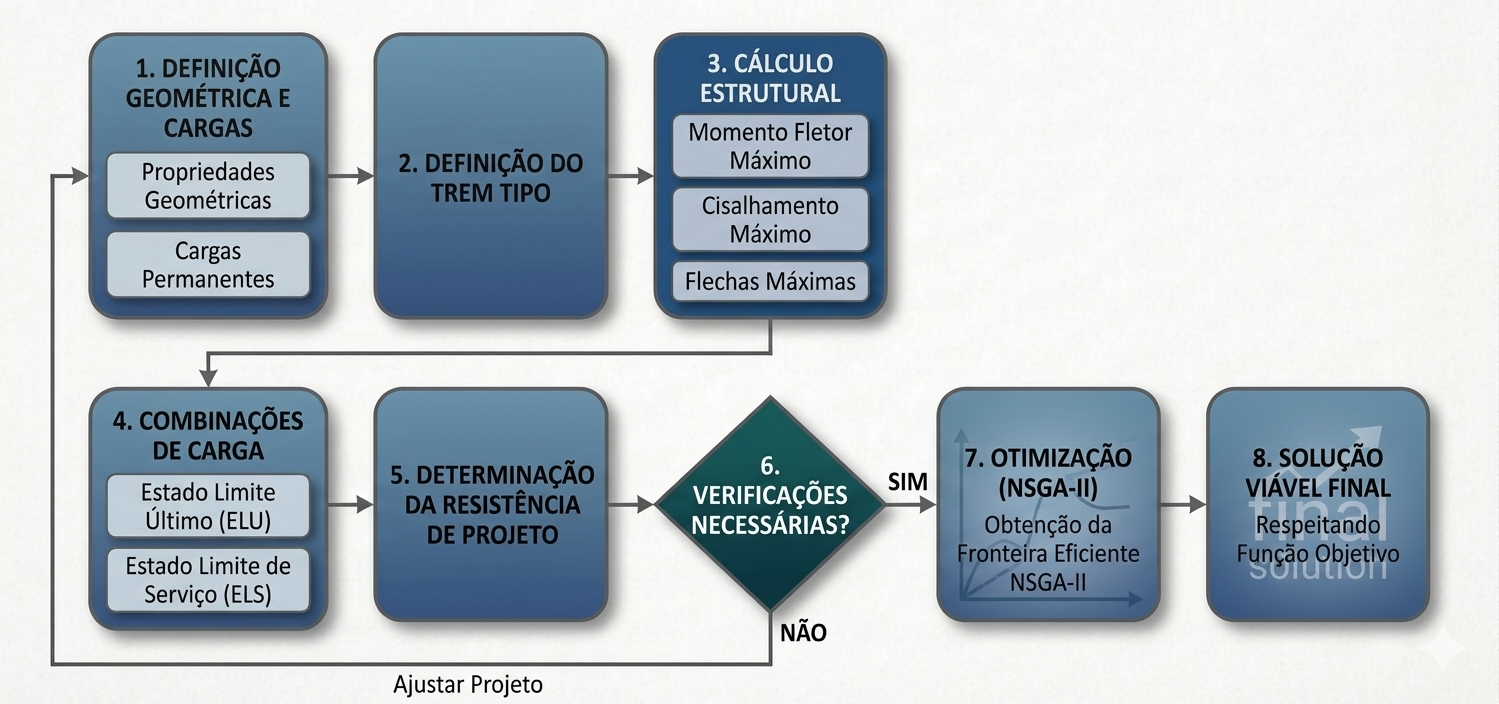
\includegraphics[width=0.8\textwidth]{imgs/fluxograma.png}
    \vspace{0.1cm}
    \par {\fontsize{11pt}{13.2pt}\selectfont \textbf{Fonte:} Autoria própria (2026).}
\end{figure}

\subsection{Dimensionamento de pontes de madeira}
% Breve intro sobre pontes de madeira (2 paragrafos no máximos). Esta ferramenta é para pontes de tal e tal jeito.


A madeira é um dos materiais mais antigos empregados na construção civil, destacando-se em pontes de pequeno e médio porte por sua elevada relação resistência-peso, durabilidade quando adequadamente tratada e baixo impacto ambiental. Em estruturas de pontes, especialmente as de madeira roliça, o material é utilizado em sua forma natural, preservando as características circulares das seções transversais e proporcionando soluções esteticamente integradas à paisagem, além de rápida execução e eficiência estrutural para vãos de até 15 metros.

O dimensionamento adequado dessas pontes exige a consideração simultânea de múltiplos critérios normativos, como os estados limites últimos e de serviço estabelecidos pela NBR 7190 \cite{NBR7190-1:2022}, além da análise de cargas permanentes e móveis (trem-tipo). A complexidade desse processo motivou o desenvolvimento de ferramentas computacionais baseadas em otimização multiobjetivo, capazes de explorar o compromisso entre a minimização do consumo de material e a maximização do desempenho estrutural, oferecendo ao projetista soluções eficientes e racionais para o projeto preliminar de pontes em madeira roliça.



\subsubsection{Levantamento de cargas}

\subsection*{Resumo das Ações e Dimensionamento de Pontes de Madeira Roliça}

O texto aborda as etapas fundamentais para a determinação dos esforços solicitantes em pontes de madeira roliça, com foco nas ações permanentes e móveis, bem como nos coeficientes de ponderação e combinações de esforços para o dimensionamento segundo as normas brasileiras NBR 8681 e NBR 7190.

\subsubsection*{Ações Permanentes}
Segundo a \textcite{NBR8681:2025}, as ações permanentes atuam continuamente ao longo da vida útil da estrutura. Em pontes de madeira roliça, incluem-se o peso próprio de elementos como longarinas, tabuleiro e rodeiros. O cálculo é realizado pela Equação~\eqref{eq:acoes_permanentes_resumo}, em função da geometria e do peso específico dos materiais.
\begin{equation}
G = \gamma \cdot A
\label{eq:acoes_permanentes_resumo}
\end{equation}
Onde:
\begin{itemize}
    \item $G$: Peso próprio (kN/m);
    \item $\gamma$: Peso específico do material (kN/m³);
    \item $A$: Área da seção transversal (m²).
\end{itemize}

\subsubsection*{Ações Móveis (Trem-Tipo)}
A carga móvel rodoviária é definida pela \textcite{nbr7188}. Os principais modelos são:
\begin{itemize}
    \item \textbf{TB-450}: Veículo-tipo com peso total de 450 kN (6 rodas de 75 kN), três eixos espaçados em 1,5 m, ocupando 18,0 m², com carga de multidão de 5 kN/m².
    \item \textbf{TB-240}: Carga mínima para estradas vicinais, com peso total de 240 kN (6 rodas de 40 kN), três eixos espaçados em 1,5 m, ocupando 18,0 m², com carga de multidão de 4 kN/m².
\end{itemize}

Para considerar os efeitos dinâmicos da passagem do veículo, aplica-se o \textbf{Coeficiente de Impacto Vertical (CIV)}, conforme as Equações \eqref{eq:CIV10_resumo} e \eqref{eq:CIVmaior_resumo}.
\begin{equation}
CIV = 1{,}35 \quad \text{para } L \leq 10{,}0 \text{ m}
\label{eq:CIV10_resumo}
\end{equation}
\begin{equation}
CIV = 1 + 1{,}06 \left( \frac{20}{LIV + 50} \right) \quad \text{para } 10{,}0 < L \leq 200{,}0 \text{ m}
\label{eq:CIVmaior_resumo}
\end{equation}
Onde $LIV$ é o comprimento característico da estrutura.





% \subsubsection{Combinações}

\subsubsection{Combinações de Ações e Verificações de Segurança}

Para a verificação da segurança e do desempenho em serviço de estruturas de madeira, torna-se necessário estabelecer critérios adequados para a combinação das ações atuantes, considerando tanto os Estados Limite Último (ELU) quanto os Estados Limite de Serviço (ELS). A NBR 7190 \textcite{NBR7190-1:2022} define procedimentos específicos para essa finalidade, levando em conta as particularidades do material madeira, como a variabilidade de suas propriedades e seu comportamento reológico diferenciado, notadamente a deformação progressiva ao longo do tempo.

\subsection{Coeficientes de Ponderação das Ações Permanentes}

Previamente à definição das combinações de ações, é necessário conhecer os esforços solicitantes característicos atuantes na estrutura. A NBR 7190 \parencite{NBR7190-1:2022} estabelece os coeficientes de ponderação $\gamma_{g}$ a serem aplicados às ações permanentes, apresentando três conjuntos de valores possíveis, cuja escolha fica a critério do projetista em função do nível de segurança pretendido, conforme discriminado a seguir:

\begin{enumerate}[label=\alph*)]
    \item $\gamma_{g} = 1,3;\ \gamma_{g} = 1,2;\ \gamma_{g} = 1,15;$ para elementos estruturais de madeira em geral;
    \item $\gamma_{g} = 1,25;\ \gamma_{g} = 1,15;\ \gamma_{g} = 1,10;$ para elementos estruturais industrializados de madeira;
\end{enumerate}

\subsection{Combinações para o Estado Limite Último (ELU)}

Para a verificação da segurança estrutural no domínio do Estado Limite Último (ELU), a NBR 7190 \parencite{NBR7190-1:2022} remete à NBR 8681 \parencite{NBR8681:2025}. Adota-se, nesse contexto, a combinação última normal, que contempla situações com probabilidade de ocorrência suficientemente elevada durante a vida útil da estrutura. A expressão geral para essa combinação é apresentada na Equação \eqref{eq:2.01}.

\begin{equation}
F_d = \sum_{i=1}^{m} \gamma_{gi}\, F_{Gi,k}
      + \gamma_{q1}\, F_{Q1,k}
      + \sum_{j=2}^{n} \gamma_{qj}\, F_{Qj,k}\, \psi_{0j}
       \label{eq:2.01}
\end{equation}

Onde:

\begin{tabular}{ll}
$F_d$            & valor de cálculo da ação combinada; \\
$\gamma_{gi}$    & coeficiente de majoração das ações permanentes; \\
$F_{G i,k}$      & valor característico das ações permanentes; \\
$\gamma_{q1}$    & coeficiente de majoração da ação variável principal; \\
$F_{Q1,k}$       & valor característico da ação variável principal; \\
$\gamma_{qj}$    & coeficiente de majoração das ações variáveis secundárias; \\
$\psi_{0j}$      & fator de combinação das ações variáveis secundárias; \\
$F_{Qj,k}$       & valor característico das ações variáveis secundárias; \\
$m$, $n$         & números de ações permanentes e de ações variáveis consideradas.
\end{tabular}

No âmbito do presente estudo, adotou-se a combinação última normal em conformidade com a NBR 7190 \parencite{NBR7190-1:2022}. Para o dimensionamento da longarina de madeira, considerou-se o trem-tipo como ação variável principal. Nesse contexto, aplicou-se a redução prevista na norma ao valor característico dessa ação, resultando na expressão apresentada na Equação \eqref{eq:2.09}. Tal redução é aplicada exclusivamente às verificações dos elementos estruturais de madeira.

\begin{equation}
      F_d = \sum_{i=1}^{m} \gamma_{gi}\, F_{Gi,k}
      + \gamma_{qw}\, 0{,}75\, F_{Qw,k}
      + \gamma_{q2}\, \psi_{0,q2}\, F_{Q2,k}
      \label{eq:2.09}
\end{equation}

Onde:

\begin{tabular}{ll}
$\gamma_{qw}$    & coeficiente de majoração da ação do vento; \\
$\gamma_{q2}$    & coeficiente de majoração da ação variável secundária; \\
$\psi_{0,q2}$    & fator de combinação da ação variável secundária; \\
$F_{Qw,k}$       & valor característico da ação do vento; \\
$F_{Q2,k}$       & valor característico da ação variável secundária.
\end{tabular}

\subsection{Combinações para o Estado Limite de Serviço (ELS)}

Objetivando garantir condições adequadas de utilização, durabilidade e conforto aos usuários, as estruturas de madeira devem ser verificadas quanto aos Estados Limite de Serviço (ELS). Essas verificações visam evitar deformações ou deslocamentos excessivos que possam comprometer a funcionalidade da construção, causar danos estéticos ou induzir vibrações indesejáveis. A NBR 7190 \parencite{NBR7190-1:2022} estabelece, para tanto, critérios associados à deformabilidade da estrutura, considerando dois cenários distintos: os deslocamentos instantâneos ($\delta_{\mathrm{inst}}$) e os deslocamentos finais ou efetivos ($\delta_{\mathrm{fin}}$).

A madeira distingue-se de outros materiais estruturais por apresentar deformação significativa ao longo do tempo sob carregamento constante, fenômeno conhecido como fluência. Em função desse comportamento reológico, as verificações de serviço devem considerar separadamente os efeitos imediatos e os efeitos diferidos.

Para a avaliação das flechas instantâneas ($\delta_{\mathrm{inst}}$), que correspondem às deformações imediatas da estrutura desconsiderando os efeitos da fluência, adota-se a combinação rara de serviço, conforme estabelecido pela NBR 8681 \parencite{NBR8681:2025}. O cálculo desses deslocamentos é realizado conforme a Equação \eqref{eq:flecha_inst}.

\begin{equation}
\delta_{\mathrm{inst}} =
\sum_{i=1}^{m} \delta_{\mathrm{inst},G_i,k}
+ \delta_{\mathrm{inst},Q_1,k}
+ \sum_{j=2}^{n} \delta_{\mathrm{inst},Q_j,k} \cdot \psi_{1,j}
\label{eq:flecha_inst}
\end{equation}

Onde:

\begin{tabular}{ll}
$\delta_{\mathrm{inst},G_i,k}$ & flechas instantâneas decorrentes das ações permanentes; \\
$\delta_{\mathrm{inst},Q_1,k}$ & flecha instantânea associada à ação variável principal; \\
$\delta_{\mathrm{inst},Q_j,k}$ & flechas instantâneas decorrentes das ações variáveis secundárias; \\
$\psi_{1,j}$ & fator de redução correspondente à combinação frequente.
\end{tabular}

Para a avaliação das flechas finais ($\delta_{\mathrm{fin}}$), que incorporam os efeitos da fluência da madeira, a NBR 7190 \parencite{NBR7190-1:2022} prescreve a utilização da combinação quase permanente de ações, conforme a Equação \eqref{eq:flecha_fin}.

\begin{equation}
\delta_{\mathrm{fin}} =
\sum_{i=1}^{m} \delta_{\mathrm{fin},G_i,k}
+ \sum_{j=1}^{n} \delta_{\mathrm{fin},Q_j,k}
\label{eq:flecha_fin}
\end{equation}

Onde:

\begin{tabular}{ll}
$\delta_{\mathrm{fin},G_i,k}$ & flechas finais associadas às ações permanentes; \\
$\delta_{\mathrm{fin},Q_j,k}$ & flechas finais associadas às ações variáveis, calculadas conforme as Equações \eqref{eq:flecha_fin_G} e \eqref{eq:flecha_fin_Q}.
\end{tabular}

As parcelas de flecha final decorrentes das ações permanentes e variáveis são obtidas, respectivamente, por meio das expressões:

\begin{equation}
\delta_{\mathrm{fin},G_i,k}
=
\delta_{\mathrm{inst},G_i,k}
+ \delta_{\mathrm{creep}}
=
\delta_{\mathrm{inst},G_i,k} \cdot (1 + \varphi)
\label{eq:flecha_fin_G}
\end{equation}

\begin{equation}
\delta_{\mathrm{fin},Q_j,k}
=
\delta_{\mathrm{inst},Q_j,k}
+ \delta_{\mathrm{creep}}
=
\delta_{\mathrm{inst},Q_j,k} \cdot \psi_{2} \cdot (1 + \varphi)
\label{eq:flecha_fin_Q}
\end{equation}

Onde:

\begin{tabular}{ll}
$\delta_{\mathrm{creep}}$ & parcela da flecha associada aos efeitos da fluência da madeira; \\
$\varphi$ & coeficiente de fluência da madeira, definido conforme o Quadro \ref{qua:fluencia}; \\
$\psi_{2}$ & fator de redução correspondente à combinação quase permanente.
\end{tabular}

O coeficiente de fluência ($\varphi$) é determinado em função do tipo de material empregado e da classe de umidade à qual a estrutura está exposta. Observa-se que classes de umidade mais elevadas implicam maiores deformações diferidas, conforme os valores apresentados no Quadro \ref{qua:fluencia}.

\clearpage
\begin{quadro}[htpb!]
    \centering
    % Define o nome como Quadro para este elemento específico
    \renewcommand{\tablename}{Quadro}
    
    % Configura o negrito e o tamanho 11pt para a Legenda (no topo)
    \captionsetup{
        labelfont={bf,small}, 
        font={small},
        labelsep=endash
    }
    \caption{Coeficiente de fluência ($\varphi$).}
    \label{qua:fluencia}

    % Definição do quadro (formato fechado) com tamanho 11pt
    \fontsize{11pt}{13.2pt}\selectfont
    \begin{tabular}{|>{\centering\arraybackslash}m{6.0cm}|>{\centering\arraybackslash}m{2.5cm}|>{\centering\arraybackslash}m{2.5cm}|>{\centering\arraybackslash}m{2.5cm}|}
        \hline
        \textbf{Materiais} & \multicolumn{3}{c|}{\textbf{Classe de umidade}} \\ \cline{2-4} 
         & \textbf{(1)} & \textbf{(2 e 3)} & \textbf{(4)} \\ \hline
        Madeira serrada, MLC, MLCC, LVL e roliça & 0,6 & 0,8 & 2,0\textsuperscript{a} \\ \hline
        Compensado estrutural & 0,8 & 1,0 & 2,5 \\ \hline
        OSB estrutural & 1,5 & 2,25 & -- \\ \hline
    \end{tabular}

    % Notas e Fonte com tamanho 11pt
    \vspace{0.1cm}
    \par {\fontsize{11pt}{13.2pt}\selectfont \textsuperscript{a} Não é permitido o uso de MLCC para a classe de umidade 4.}
    
    \par {\fontsize{11pt}{13.2pt}\selectfont \textbf{Fonte:} Adaptado da NBR 7190 \parencite{NBR7190-1:2022}.}
\end{quadro}

\subsubsection{Propriedades da madeira}

A determinação das propriedades geométricas da seção transversal constitui uma etapa fundamental na análise e no dimensionamento de elementos estruturais, uma vez que essas propriedades influenciam diretamente a resistência, a rigidez e a estabilidade da estrutura. Parâmetros como área, momento de inércia, módulo resistente e raio de giração são essenciais para a verificação dos estados limites últimos e de serviço, conforme os critérios estabelecidos pela NBR 7190 \cite{NBR7190-1:2022}.

Para o caso de seções transversais circulares maciças, a área (m²) pode ser obtida conforme a Equação~\eqref{eq:1}.

\begin{equation}
A = \frac{\pi d^2}{4}
\label{eq:1}
\end{equation}

Onde, \(d\) é o diâmetro da seção transversal (m).

Por sua vez, para seções transversais de geometria retangular, a área (m²) é determinada pela Equação~\eqref{eq:2}.

\begin{equation}
A = b \cdot h
\label{eq:2}
\end{equation}

Onde, \(b\) corresponde à largura (m) e \(h\) à sua altura (m).

Os momentos de inércia em relação aos eixos principais ($m^4$) caracterizam a distribuição da área da seção transversal e são determinantes para a avaliação da rigidez à flexão dos elementos estruturais. Esses parâmetros dependem diretamente da geometria da seção analisada.

Para seções transversais circulares maciças, em razão da simetria geométrica, os momentos de inércia ($m^4$) em relação aos eixos principais \(x\) e \(y\) são idênticos, sendo expressos pela Equação~\eqref{eq:3}.

\begin{equation}
I_x = I_y = \frac{\pi d^4}{64}
\label{eq:3}
\end{equation}

Onde, \(d\) representa o diâmetro da seção (m).

Por sua vez, para seções transversais de geometria retangular, como o tabuleiro, os momentos de inércia ($m^4$) em relação aos eixos principais são distintos e definidos pelas Equações \eqref{eq:4} e \eqref{eq:5}.

\begin{equation}
I_x = \frac{b h^3}{12}
\label{eq:4}
\end{equation}

\begin{equation}
I_y = \frac{h b^3}{12}
\label{eq:5}
\end{equation}

Onde, \(b\) corresponde à largura (m)  e \(h\) à sua altura (m).

O módulo resistente (m³) está associado à capacidade da seção transversal em resistir aos momentos fletores máximos, sendo definido como a razão entre o momento de inércia e a distância da fibra mais afastada ao eixo neutro. Para seções circulares, o módulo resistente é o mesmo em ambos os eixos principais e é dado pela Equação~\eqref{eq:6}.

\begin{equation}
W_x = W_y = \frac{I_x}{d/2}
\label{eq:6}
\end{equation}

Já para seções retangulares, os módulos resistentes (m³) em relação aos eixos principais são definidos pelas Equações \eqref{eq:7} e \eqref{eq:8}.

\begin{equation}
W_x = \frac{I_x}{h/2}
\label{eq:7}
\end{equation}

\begin{equation}
W_y = \frac{I_y}{b/2}
\label{eq:8}
\end{equation}

Outro parâmetro relevante é o raio de giração (m), amplamente utilizado nas verificações de estabilidade estrutural, como a análise de flambagem. O raio de giração relaciona o momento de inércia com a área da seção transversal. Para seções circulares e retangulares, os raios de giração são expressos pelas Equações \eqref{eq:9} e \eqref{eq:10}.

\begin{equation}
r_x = \sqrt{\frac{I_x}{A}}
\label{eq:9}
\end{equation}

\begin{equation}
r_y = \sqrt{\frac{I_y}{A}}
\label{eq:10}
\end{equation}

Dessa forma, a determinação das propriedades geométricas das seções transversais circulares e retangulares fornece a base necessária para a realização das verificações estruturais, assegurando coerência entre a modelagem geométrica adotada e os critérios normativos aplicáveis.

reescreva com outras palavras, mantenha no formado de latex 

\subsubsection{Dimensionamento à flexão}

A NBR 7190 \parencite{NBR7190-1:2022} exige que a verificação da flexão simples em peças estruturais de madeira considere a possibilidade de flexão reta ou flexão oblíqua, conforme a orientação do carregamento em relação aos eixos principais de inércia da seção transversal.

No caso da flexão reta, o momento fletor atua em torno de apenas um eixo principal, gerando uma distribuição linear das tensões normais. A verificação é feita comparando-se a tensão de flexão de cálculo com a resistência de cálculo ao momento fletor, conforme apresentado na Equação~\eqref{eq:flexao_reta}.

\begin{equation}
\frac{\sigma_{Mx,d}}{f_{m,d}} = \frac{M_d}{W \, f_{m,d}} \leq 1
\label{eq:flexao_reta}
\end{equation}

Onde:

\begin{tabular}{ll}
$\sigma_{Mx,d}$ & Tensão atuante de cálculo referente à flexão em torno do eixo $x$ (kPa);\\
$f_{m,d}$ & Resistência de cálculo à flexão da madeira (kPa);\\
$M_d$ & Momento fletor solicitante de cálculo (kN.m);\\
$W_x$ & Módulo de resistência elástico da seção em relação ao eixo $x$ ($m^3$);\\
\end{tabular}

\subsection{Método de otimização multiobjetivo}

O projeto da ponte de madeira é integrado a uma estrutura de otimização multiobjetivo visando apoiar uma etapa racional e orientada ao desempenho do dimensionamento estrutural. A tarefa de otimização é formulada como um problema de otimização multiobjetivo e resolvida por meio do Algoritmo Genético de Ordenação Não Dominada II (NSGA-II), sendo adequado para problemas não lineares, com restrições e objetivos conflitantes.

Um problema de otimização multiobjetivo envolve a minimização e/ou maximização simultânea de múltiplas funções objetivo, sujeitas a um conjunto de restrições que definem a viabilidade das soluções candidatas. Diferentemente da otimização monoobjetivo ele não conduz a uma única solução ótima, alternativamente, resulta em um conjunto de soluções ótimas de Pareto, cada uma representando um caso distinto entre critérios de desempenho concorrentes.

A formulação matemática geral de um problema de otimização multiobjetivo pode ser expressa conforme a Equação~\eqref{eq:mop}.

\begin{equation}
\begin{cases} 
f_m(\mathbf{x}), & m = 1,2,\ldots,M; \\ 
g_j(\mathbf{x}) \leq 0, & j = 1,2,\ldots,J; \\ 
h_k(\mathbf{x}) = 0, & k = 1,2,\ldots,K; \\ 
x_i^{(L)} \leq x_i \leq x_i^{(U)}, & i = 1,2,\ldots,n.
\end{cases}
\label{eq:mop}
\end{equation}

Nesta formulação, o vetor de funções objetivo é definido segundo a Equação~\eqref{eq:fx}.

\begin{equation}
f(\mathbf{x}) = \left(f_1(\mathbf{x}), f_2(\mathbf{x}), \ldots, f_M(\mathbf{x})\right)^T
\label{eq:fx}
\end{equation}

Onde, $\mathbf{x} = (x_1, x_2, \ldots, x_n)^T$ representa o vetor $n$-dimensional de variáveis de projeto. 

O espaço de projeto viável é restringido por restrições de desigualdade $g_j(\mathbf{x})$, restrições de igualdade $h_k(\mathbf{x})$ e restrições de domínio definidas pelos limites inferior e superior $x_i^{(L)}$ e $x_i^{(U)}$, que em conjunto definem o domínio admissível $(D)$ \parencite{DEB2009}.

Objetivos inicialmente formulados como problemas de maximização são convertidos em problemas equivalentes de minimização por meio da multiplicação das respectivas funções objetivo por $-1$, garantindo uma estrutura de otimização unificada e consistente.

A Figura~\ref{fig:pareto} ilustra o espaço de soluções de um problema biobjetivo, destacando a diversidade de soluções viáveis e o conceito de dominância de Pareto que caracteriza a otimização multiobjetivo.

\begin{figure}[htpb!]
    \centering
    \captionsetup{
        labelfont={bf,small}, 
        font={small},
        labelsep=endash
    }
    \caption{Possíveis soluções de um problema de otimização multiobjetivo.}
    \label{fig:pareto} 
    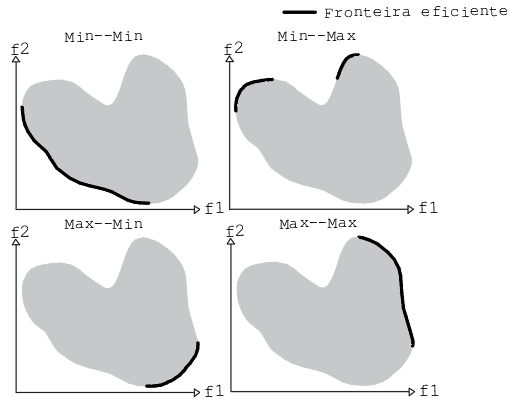
\includegraphics[width=0.6\textwidth]{imgs/z_types_frontier.png}
    \vspace{0.1cm}
    \par {\fontsize{11pt}{13.2pt}\selectfont \textbf{Fonte:} {\textcite{DEB2009}.}
 \end{figure}


 
 \subsection{Algoritmo Genético de Ordenação Não Dominada II (NSGA-II)}

 O problema de otimização multiobjetivo é resolvido utilizando o Algoritmo Genético de Ordenação Não Dominada II (NSGA-II), um algoritmo evolutivo desenvolvido especificamente para aproximar o conjunto ótimo de Pareto em problemas que envolvem objetivos conflitantes \parencite{DEB2009}. Diferentemente de abordagens baseadas em escalarização, o NSGA-II preserva a natureza multiobjetivo do problema e busca um conjunto diverso de soluções não dominadas.

Seja $f(\mathbf{x}) = \left(f_1(\mathbf{x}), f_2(\mathbf{x}), \ldots, f_M(\mathbf{x})\right)^T$ o vetor de funções objetivo. Dadas duas soluções candidatas $\mathbf{x}^a$ e $\mathbf{x}^b$, diz-se que $\mathbf{x}^a$ \textit{domina no sentido de Pareto} $\mathbf{x}^b$, denotado por $\mathbf{x}^a \prec \mathbf{x}^b$, se atende as condições da Equação \eqref{eq:333}.

\begin{equation}
\forall m \in \{1,\ldots,M\}, \; f_m(\mathbf{x}^a) \leq f_m(\mathbf{x}^b)
\quad \text{e} \quad
\exists m \; : \; f_m(\mathbf{x}^a) < f_m(\mathbf{x}^b)
\label{eq:333}
\end{equation}

A cada geração, a população é ordenada em frentes sucessivas não dominadas $\mathcal{F}_1, \mathcal{F}_2, \ldots$, sendo $\mathcal{F}_1$ o conjunto de soluções não dominadas, representando a aproximação atual da fronteira de Pareto. A seleção dos indivíduos é baseada tanto na hierarquia de Pareto quanto na diversidade das soluções.

Para preservar a diversidade ao longo da fronteira de Pareto, o NSGA-II emprega a métrica denominada distância de aglomeração (\textit{crowding distance}). Para uma solução $\mathbf{x}_i$ pertencente a uma determinada frente, a distância de aglomeração $d_i$ é calculada conforme a Equação~\eqref{eq:diversidade}.

\begin{equation}
d_i = \sum_{m=1}^{M}
\frac{f_m(\mathbf{x}_{i+1}) - f_m(\mathbf{x}_{i-1})}
{f_m^{\max} - f_m^{\min}}
\label{eq:diversidade}
\end{equation}

Onde, $f_m^{\max}$ e $f_m^{\min}$ representam, respectivamente, os valores máximo e mínimo da $m$-ésima função objetivo dentro da mesma frente. Soluções localizadas em regiões menos densas do espaço de objetivos são preferidas, promovendo uma distribuição uniforme da fronteira eficiente.

Uma estratégia elitista é adotada por meio da combinação das populações parental e descendente, sendo os melhores indivíduos selecionados com base no nível de Pareto e na distância de aglomeração. O resultado final do processo de otimização é uma aproximação da fronteira eficiente de Pareto, representando um conjunto de alternativas de projeto viáveis, nas quais a melhoria de um objetivo implica necessariamente a degradação de pelo menos outro.

\subsection{Tratamento das restrições}

O tratamento das restrições a base de otimização multiobjetivo propõe uma abordagem baseada em viabilidade, conforme implementado na Biblioteca de otimização \texttt{pymoo} \parencite{blank2020}. Dessa forma, o problema de otimização multiobjetivo com restrições é definido por um conjunto de restrições de desigualdade e igualdade, expressas, respectivamente, segundo as Equações \eqref{eq:g} e \eqref{eq:h}.

\begin{equation}
g_j(\mathbf{x}) \leq 0, \quad j = 1,2,\ldots,J
\label{eq:g}
\end{equation}

e

\begin{equation}
h_k(\mathbf{x}) = 0, \quad k = 1,2,\ldots,K
\label{eq:h}
\end{equation}

As restrições de igualdade são internamente transformadas em restrições de desigualdade por meio da introdução de uma tolerância numérica $\varepsilon$, conforme a expressão \eqref{eq:hk}.

\begin{equation}
|h_k(\mathbf{x})| - \varepsilon \leq 0
\label{eq:hk}
\end{equation}

Para cada solução candidata $\mathbf{x}$, é calculada uma medida agregada de violação das restrições $\mathrm{CV}(\mathbf{x})$, segundo a Equação~\eqref{eq:sum}.

\begin{equation}
\mathrm{CV}(\mathbf{x}) =
\sum_{j=1}^{J} \max\left(0, g_j(\mathbf{x})\right)
+
\sum_{k=1}^{K} \max\left(0, |h_k(\mathbf{x})| - \varepsilon \right)
\label{eq:sum}
\end{equation}

Uma solução é considerada viável se $\mathrm{CV}(\mathbf{x}) = 0$, sendo considerada inviável caso contrário. Durante o processo evolutivo, a comparação e seleção das soluções seguem as regras de viabilidade originalmente propostas por \textcite{DEB2009}. De acordo com essas regras, soluções viáveis sempre dominam soluções inviáveis; entre soluções viáveis, aplica-se a dominância de Pareto; e, entre soluções inviáveis, a ordenação é baseada no grau total de violação das restrições \parencite{DEB2009}.

Essa estratégia orientada pela viabilidade permite que o processo de otimização convirja de forma consistente e numericamente robusta para a fronteira de Pareto viável, sem a necessidade de funções de penalização ou reformulação das funções objetivo, sendo particularmente adequada para problemas de otimização estrutural com múltiplos objetivos e restrições rigorosas \parencite{blank2020}.

% This section outlines the framework development process and demonstrates its application through parametric structural design. The methodology is organized as follows: \textbf{a) Structural Modeling Approach}, presenting the beam conceptualization and internal load analysis for the adopted simply supported beam configuration; \textbf{b) Design of timber elements}, detailing the verification equations for bending moment, shear, and displacement compliance with NBR 7190 standards; and \textbf{c) Optimization Process}, describing the objective functions and constraint formulations. Figure~\ref{fig:z_flux_data_framework} illustrates the overall framework workflow.

% \subsection{Illustrative examples}
% Esta seção descreve os locais de instalação das pontes que serão objeto de projeto neste software. As estruturas em questão, situadas no município de Ipameri, encontram-se em estado precário, demandando intervenção urgente.
% Com o objetivo de subsidiar a análise estrutural e a caracterização espacial para os futuros projetos, foram realizadas visitas técnicas de inspeção a três pontes na região. Os dados e observações coletados in loco são detalhados a seguir na tabela \ref{tab:classes_resistencia}.


% % Tabela
% % Local, latitude, longitude, altitude, vão da pista, vão livre, Rodovia, carga permanente (se tem capa asfáltica) kN/m²

% \renewcommand{\arraystretch}{2}
% \begin{table}[htbp]
% \captionsetup{position=top}
% \centering
% \caption{Características Técnicas e Georreferenciamento das Pontes Inspecionadas em Ipameri.}
% \label{tab:classes_resistencia}
% \footnotesize
% \begin{tabular}{>{\centering\arraybackslash}p{2 cm} 
%                 >{\centering\arraybackslash}p{4.5 cm}
%                 >{\centering\arraybackslash}p{4.5 cm}
%                 >{\centering\arraybackslash}p{4.5 cm}}
% \hline
% \textbf{Pontes} & \textbf{ Rio do Braço} & \textbf{Três Bocas} & \textbf{ Mascarenhas de Morais} \\\hline

% \raisebox{6\height}{\textbf{Ilustração}}
% & 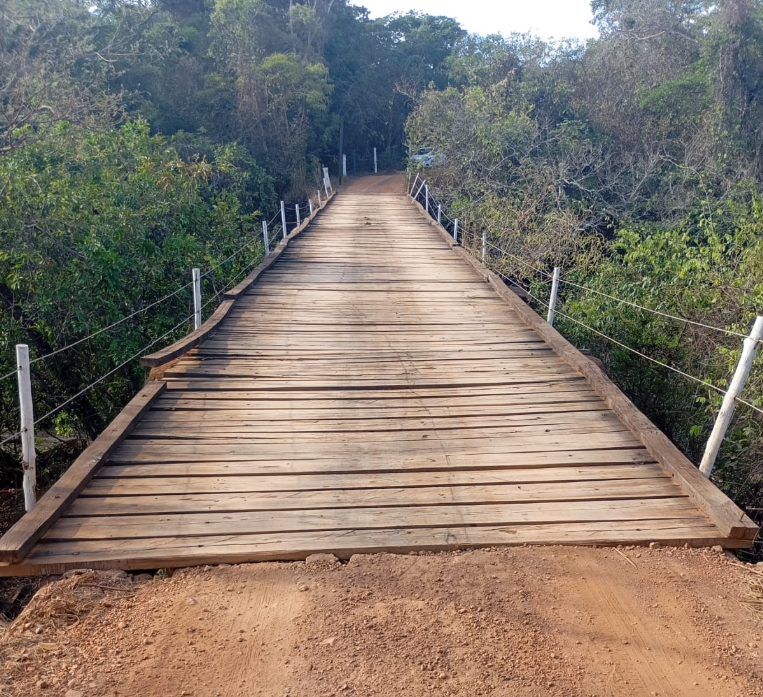
\includegraphics[width=3.3cm]{imgs/Rio do Braço.png} 
% & 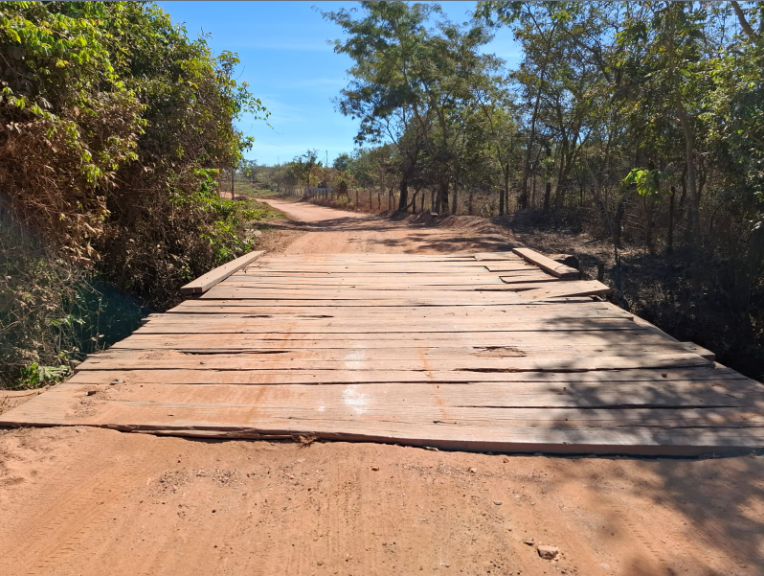
\includegraphics[width=4cm]{imgs/Tres bocas.png}
% & 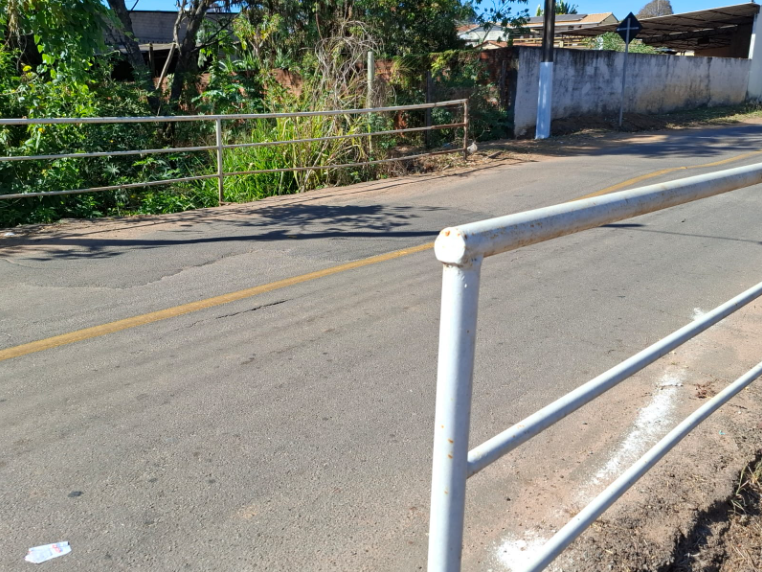
\includegraphics[width=4cm]{imgs/Mascarenha de morais.png} \\%\hline

% \textbf{Localização} & Estra. Prainha & Estra. Acesso ao Ribe. Três Bocas & Rua Masc. de Morais \\%\hline

% \textbf{Latitude} & -17°45’03.5" & -17°75’43.71" & -17°43’53.5" \\%\hline

% \textbf{Longitude} & -48°09’55.2" & -48°18’43.90" & 48°09’54.9" \\%\hline

% \textbf{Altitude} & 668 m & 682 m & 739 m \\%\hline

% \textbf{Comprimento} & 13,4 m & 6,4 m & 7 m \\%\hline

% \textbf{Largura } & 3,5 m & 3,5 m & 7 m \\%\hline

% \textbf{Tipo Longarinas} & Mad. Roliça & Mad. Roliça & Mad. Roliça \\%\hline

% \textbf{Massa Asfáltica} & Não Aplica & Não Aplica & 0.69 kN/m2 \\%\hline

% \textbf{Sist. Estrutural} & Biapoiado & Biapoiado & Biapoiado \\
% \hline
% \end{tabular}
% %\small Fonte: Autoria Propriá.
% \end{table}

% A tabela evidencia a heterogeneidade das estruturas inspecionadas, com variações significativas em localização geográfica, altitude e dimensão do vão. A ausência do dado de carga permanente para duas das pontes destaca uma possível limitação nos dados disponíveis ou uma diferença no método de inspeção aplicado em cada caso, informação crucial para as próximas etapas de análise estrutural.



% \begin{figure}[htbp!]
%     \centering
%     \includegraphics[width=0.5\textwidth]{z_flux_data_framework.png}
%     \caption{User interaction flowchart with the structural optimization framework.}
%     \label{fig:z_flux_data_framework}
% \end{figure}

% \subsection{Structural Modeling Approach}
% The simply supported beam configuration was adopted as the primary structural scheme due to its prevalence in practical applications. Internal force distributions were derived through classical solid mechanics formulations. Table~\ref{fig:exemplo} enumerates the complete internal load regimes and associated displacement fields under both permanent (dead) and load train conditions.

% As Equações xxx a xx rperesentam os valores máximos de mommentos

% \begin{table}[htbp!]
% \centering
% \caption{Loads and internal loads for girders.}
% \label{tab:fig_eq_examples}
% \begin{tabular}{cc}
%     \hline
%     \textbf{Schema} & \textbf{Equations} \\
%     \hline
    
%     % Linha 1
%     \begin{minipage}{0.3\textwidth}
%         \centering
%         
\includegraphics[width=1.2\linewidth]{imgs/ART./Pos. veículo-tipo.png}
%         \captionof{subfigure}{Structural configuration 1}
%         \label{fig:example1}
%     \end{minipage}
%     &
%     \begin{minipage}{0.5\textwidth}
%         \centering
%         \begin{equation}
%             M_{g,k} = \frac{g \cdot L^{2}}{8}
%             \label{eq:force12}
%         \end{equation}
%             \vspace{0.5cm}
%         \begin{equation}
%             M_{g,k} = D_{f,M} \left( \frac{3 \cdot P \cdot L}{4} - P \cdot a \right),
% \quad \text{para } 3\,\text{m} \leq L \leq 6\,\text{m}
%             \label{eq:stress1}
%         \end{equation}
%             \vspace{0.5cm}
%         \begin{equation}
%             M_{g,k} = D_{f,M} \left[ \left( \frac{3 \cdot P \cdot L}{4} - P \cdot a \right) + \frac{q \cdot c^{2}}{2} \right],\quad \text{para } L > 6\,\text{m}
%             \label{eq:force1}
%         \end{equation}
%             \vspace{0.5cm}
%         \begin{equation}
%             \delta_{g,k} = \frac{5 \cdot g \cdot L^{4}}{384 \cdot E_{M,\mathrm{ef}} \cdot I}
%         \label{eq:force1}
%         \end{equation}
%             \vspace{0.5cm}
%         \begin{equation}
%             \delta_{q,k} = D_{f,m} \cdot \frac{P}{48 \cdot E_{M,\mathrm{ef}} \cdot I}
%             \left[ L^{3} + 2 \cdot b \cdot \left( 3 \cdot L^{2} - 4 \cdot b^{2} \right) \right]
%         \label{eq:force1}
%         \end{equation}
%     \end{minipage}
%     \\
%     \hline
    
%     % Linha 2
%     \begin{minipage}{0.4\textwidth}
%         \centering
%         \includegraphics[width=0.9\linewidth]{example_fig2.png}
%         \captionof{subfigure}{Structural configuration 2}
%         \label{fig:example2}
%     \end{minipage}
%     &
%     \begin{minipage}{0.5\textwidth}
%         \centering
%         \begin{equation}
%             M = F \cdot d
%             \label{eq:moment1}
%         \end{equation}
%         \vspace{0.5cm}
%         \begin{equation}
%             \epsilon = \frac{\delta}{L}
%             \label{eq:strain1}
%         \end{equation}
%     \end{minipage}
%     \\
%     \hline
    
%     % Linha 3
%     \begin{minipage}{0.4\textwidth}
%         \centering
%         \includegraphics[width=0.9\linewidth]{example_fig3.png}
%         \captionof{subfigure}{Structural configuration 3}
%         \label{fig:example3}
%     \end{minipage}
%     &
%     \begin{minipage}{0.5\textwidth}
%         \centering
%         \begin{equation}
%             I = \frac{b \cdot h^3}{12}
%             \label{eq:inertia}
%         \end{equation}
%         \vspace{0.5cm}
%         \begin{equation}
%             \delta_{max} = \frac{5 \cdot w \cdot L^4}{384 \cdot E \cdot I}
%             \label{eq:deflection}
%         \end{equation}
%     \end{minipage}
%     \\
%     \hline
% \end{tabular}
% \end{table}

% Similarly, the internal load analysis for deck elements is summarized in Table~\ref{fig:exemplo}.

% \begin{table}[htbp!]
% \centering
% \caption{Loads and internal loads for slab deck design.}
% \label{tab:fig_eq_examples}
% \begin{tabular}{cc}
%     \hline
%     \textbf{Schema} & \textbf{Equations} \\
%     \hline
    
%     % Linha 1
%     \begin{minipage}{0.4\textwidth}
%         \centering
%         \includegraphics[width=0.9\linewidth]{example_fig1.png}
%         \captionof{subfigure}{Structural configuration 1}
%         \label{fig:example1}
%     \end{minipage}
%     &
%     \begin{minipage}{0.5\textwidth}
%         \centering
%         \begin{equation}
%             F = k \cdot \delta
%             \label{eq:force1}
%         \end{equation}
%         \vspace{0.5cm}
%         \begin{equation}
%             \sigma = \frac{F}{A}
%             \label{eq:stress1}
%         \end{equation}
%     \end{minipage}
%     \\
%     \hline
    
%     % Linha 2
%     \begin{minipage}{0.4\textwidth}
%         \centering
%         \includegraphics[width=0.9\linewidth]{example_fig2.png}
%         \captionof{subfigure}{Structural configuration 2}
%         \label{fig:example2}
%     \end{minipage}
%     &
%     \begin{minipage}{0.5\textwidth}
%         \centering
%         \begin{equation}
%             M = F \cdot d
%             \label{eq:moment1}
%         \end{equation}
%         \vspace{0.5cm}
%         \begin{equation}
%             \epsilon = \frac{\delta}{L}
%             \label{eq:strain1}
%         \end{equation}
%     \end{minipage}
%     \\
%     \hline
    
%     % Linha 3
%     \begin{minipage}{0.4\textwidth}
%         \centering
%         \includegraphics[width=0.9\linewidth]{example_fig3.png}
%         \captionof{subfigure}{Structural configuration 3}
%         \label{fig:example3}
%     \end{minipage}
%     &
%     \begin{minipage}{0.5\textwidth}
%         \centering
%         \begin{equation}
%             I = \frac{b \cdot h^3}{12}
%             \label{eq:inertia}
%         \end{equation}
%         \vspace{0.5cm}
%         \begin{equation}
%             \delta_{max} = \frac{5 \cdot w \cdot L^4}{384 \cdot E \cdot I}
%             \label{eq:deflection}
%         \end{equation}
%     \end{minipage}
%     \\
%     \hline
% \end{tabular}
% \end{table}

% \subsection{Design of timber elements} \label{sec:design_timer_member}

% \subsection{Multi-Objective Optimization Framework}

% The parametric design of the timber bridge is integrated with a multi-objective optimization framework to support a rational and performance-driven pre-sizing stage. The optimization task is formulated as a \textit{multi-objective optimization problem} (MOP) and solved using the \textit{Non-dominated Sorting Genetic Algorithm II} (NSGA-II), which is particularly suitable for nonlinear, constrained problems involving conflicting objectives.

% A multi-objective optimization problem (MOO) involves the simultaneous minimization and/or maximization of multiple objective functions, subject to a set of constraints that define the feasibility of candidate solutions. Unlike single-objective optimization, MOO does not lead to a unique optimal solution; instead, it results in a set of Pareto-optimal solutions, each representing a different compromise among competing performance criteria.

% The general mathematical formulation of a multi-objective optimization problem can be expressed as:

% \begin{equation}
% \begin{cases} 
% f_m(\mathbf{x}), & m = 1,2,\ldots,M; \\ 
% g_j(\mathbf{x}) \leq 0, & j = 1,2,\ldots,J; \\ 
% h_k(\mathbf{x}) = 0, & k = 1,2,\ldots,K; \\ 
% x_i^{(L)} \leq x_i \leq x_i^{(U)}, & i = 1,2,\ldots,n.
% \end{cases}
% \label{eq:mop}
% \end{equation}

% In this formulation, the vector of objective functions is defined as
% $f(\mathbf{x}) = \left(f_1(\mathbf{x}), f_2(\mathbf{x}), \ldots, f_M(\mathbf{x})\right)^T$,
% where $\mathbf{x} = (x_1, x_2, \ldots, x_n)^T$ denotes the $n$-dimensional vector of design variables. The feasible design space is constrained by inequality constraints $g_j(\mathbf{x})$, equality constraints $h_k(\mathbf{x})$, and bound constraints defined by the lower and upper limits $x_i^{(L)}$ and $x_i^{(U)}$, which together define the admissible design domain $D$ \cite{deb_multi-objective_2009}.

% Objectives originally formulated as maximization problems are converted into equivalent minimization problems by multiplying the corresponding objective functions by $-1$, ensuring a unified and consistent optimization framework.

% Figure~\ref{fig:pareto} illustrates the solution landscape of a bi-objective optimization problem, highlighting the diversity of feasible solutions and the concept of Pareto dominance that characterizes multi-objective optimization.

% \begin{figure}[htpb!]
%     \centering
%     
\includegraphics[width=0.8\textwidth]{./z_types_frontier.png}
%     \caption{Possible solutions of a two-dimensional multi-objective optimization problem \cite{deb_multi-objective_2009}.}
%     \label{fig:pareto}
% \end{figure}

% \subsubsection{Non-dominated Sorting Genetic Algorithm II (NSGA-II)}

% The multi-objective optimization problem is solved using the \textit{Non-dominated Sorting Genetic Algorithm II} (NSGA-II), an evolutionary algorithm specifically designed to approximate the Pareto-optimal set in problems involving conflicting objectives \cite{deb_multi-objective_2009}. Unlike scalarization-based approaches, NSGA-II preserves the multi-objective nature of the problem and seeks a diverse set of non-dominated solutions.

% Let $f(\mathbf{x}) = \left(f_1(\mathbf{x}), f_2(\mathbf{x}), \ldots, f_M(\mathbf{x})\right)^T$ denote the vector of objective functions. Given two candidate solutions $\mathbf{x}^a$ and $\mathbf{x}^b$, $\mathbf{x}^a$ is said to \textit{Pareto-dominate} $\mathbf{x}^b$, denoted by $\mathbf{x}^a \prec \mathbf{x}^b$, if
% \begin{equation}
% \forall m \in \{1,\ldots,M\}, \; f_m(\mathbf{x}^a) \leq f_m(\mathbf{x}^b)
% \quad \text{and} \quad
% \exists m \; : \; f_m(\mathbf{x}^a) < f_m(\mathbf{x}^b).
% \end{equation}

% At each generation, the population is sorted into successive non-dominated fronts $\mathcal{F}_1, \mathcal{F}_2, \ldots$, where $\mathcal{F}_1$ contains the set of non-dominated solutions and represents the current approximation of the Pareto front. Selection is based on both Pareto rank and solution diversity.

% To preserve diversity along the Pareto front, NSGA-II employs the \textit{crowding distance} metric. For a solution $\mathbf{x}_i$ within a given front, the crowding distance $d_i$ is computed as
% \begin{equation}
% d_i = \sum_{m=1}^{M}
% \frac{f_m(\mathbf{x}_{i+1}) - f_m(\mathbf{x}_{i-1})}
% {f_m^{\max} - f_m^{\min}},
% \end{equation}
% where $f_m^{\max}$ and $f_m^{\min}$ denote the maximum and minimum values of the $m$-th objective within the same front. Solutions located in less crowded regions of the objective space are preferred, promoting a well-distributed approximation of the efficient frontier.

% An elitist strategy is adopted by combining parent and offspring populations and selecting the best individuals based on Pareto rank and crowding distance. The final outcome of the optimization process is an approximation of the Pareto-efficient frontier, representing a set of feasible design alternatives in which improvement in one objective necessarily leads to deterioration in at least one other.

% In the present study, NSGA-II is embedded within a parametric digital twin of the timber bridge, enabling iterative evaluation of candidate solutions through the structural model. This integration allows an efficient exploration of the design space and provides a robust basis for subsequent decision-making and reliability-based analyses.

% \subsubsection{Handling Constraints}

% Constraint handling in the proposed multi-objective optimization framework follows a feasibility-based approach, as implemented in the \texttt{pymoo} optimization library \cite{blank2020}. The constrained multi-objective optimization problem is defined by a set of inequality and equality constraints, expressed respectively as:

% \begin{equation}
% g_j(\mathbf{x}) \leq 0, \quad j = 1,2,\ldots,J,
% \end{equation}
% and
% \begin{equation}
% h_k(\mathbf{x}) = 0, \quad k = 1,2,\ldots,K.
% \end{equation}

% Equality constraints are internally transformed into inequality constraints by introducing a numerical tolerance $\varepsilon$, such that:

% \begin{equation}
% |h_k(\mathbf{x})| - \varepsilon \leq 0.
% \end{equation}

% For each candidate solution $\mathbf{x}$, an aggregated constraint violation measure $\mathrm{CV}(\mathbf{x})$ is computed as
% \begin{equation}
% \mathrm{CV}(\mathbf{x}) =
% \sum_{j=1}^{J} \max\left(0, g_j(\mathbf{x})\right)
% +
% \sum_{k=1}^{K} \max\left(0, |h_k(\mathbf{x})| - \varepsilon \right).
% \end{equation}

% A solution is considered feasible if $\mathrm{CV}(\mathbf{x}) = 0$ and infeasible otherwise. During the evolutionary search, solution comparison and selection are governed by feasibility rules originally proposed by Deb. According to these rules, feasible solutions always dominate infeasible ones, Pareto dominance is applied among feasible solutions, and infeasible solutions are ranked based on their total constraint violation \cite{deb_multi-objective_2009}.

% This feasibility-driven strategy allows the optimization process to converge toward the feasible Pareto front in a consistent and numerically robust manner, without the need for penalty functions or objective reformulation, and is particularly suitable for structural optimization problems involving multiple competing objectives and strict design constraints \cite{blank2020}.

% \subsubsection{Build optimization for timber design}

% This section presents the formulation of the multi-objective optimization problem adopted for the structural pre-sizing of the timber bridge system. The optimization problem is fully coupled with the parametric structural model and aims at identifying efficient trade-off solutions that satisfy both structural safety and serviceability requirements.

% The structural system under consideration consists of a timber deck composed of longitudinal boards supported by circular timber girders (stringers), regularly spaced at a distance $\mathrm{esp}$. The deck is subjected to permanent actions (dead load), including its self-weight, and variable actions associated with traffic loading (live load, train load). The resulting loads acting on the deck are transferred to the supporting girders and modeled as uniformly distributed loads along their span.

% A schematic representation of the structural system and load transfer mechanism is provided in Figure~\ref{fig:structural_system}. Detailed expressions for internal forces, stresses, and deflections in both the deck and the girders are presented in Section~\ref{sec:design_timer_member}.

% \begin{figure}[htpb!]
%     \centering
%     % Placeholder figure
%     \fbox{
%         \parbox[c][6cm][c]{0.85\textwidth}{
%             \centering
%             \vspace{0.5cm}
%             \textbf{Schematic representation of the timber bridge structural system}\\[0.5cm]
%             Timber deck boards supported by circular timber girders\\
%             uniformly spaced by $\mathrm{esp}$\\[0.5cm]
%             Dead load (self-weight) and live load (train load) acting on the deck\\
%             and transferred as distributed loads to the girders
%             \vspace{0.5cm}
%         }
%     }
%     \caption{Conceptual representation of the timber bridge structural system, illustrating the timber deck supported by circular girders spaced by $\mathrm{esp}$, as well as the load transfer mechanism from the deck to the supporting elements.}
%     \label{fig:structural_system}
% \end{figure}


% \paragraph{Design variables}

% The optimization problem is defined in terms of a vector of design variables $\mathbf{x}$, which includes the geometric parameters of the circular timber girder and, when applicable, additional structural parameters governing the deck--girder interaction. In particular, the cross-sectional properties of the girder are functions of its diameter, which directly controls stiffness, strength, and self-weight.

% \paragraph{Objective functions}

% The optimization problem is formulated with two conflicting objective functions.

% The first objective consists of minimizing the cross-sectional area of the circular timber girder, defined as
% \begin{equation}
% f_1(\mathbf{x}) = A_g,
% \end{equation}
% where $A_g$ denotes the cross-sectional area of the girder. This objective is directly related to material consumption and structural weight.

% The second objective aims at maximizing the structural performance associated with serviceability, expressed through a displacement-based performance function. For consistency with the minimization framework, this objective is defined as
% \begin{equation}
% f_2(\mathbf{x}) = - \frac{\delta_{\mathrm{tot}}}{\delta_{\mathrm{lim}}},
% \end{equation}
% where $\delta_{\mathrm{tot}}$ is the total mid-span deflection of the girder under combined dead and live loads, and $\delta_{\mathrm{lim}} = L/250$ represents the admissible serviceability limit, with $L$ being the span length of the girder.

% \paragraph{Constraints}

% The optimization problem is subject to structural constraints associated with strength and serviceability requirements of both the girder and the deck.

% For the timber girder, the following constraints are imposed:

% \begin{itemize}
%     \item \textit{Bending stress constraint}:
%     \begin{equation}
%     g_{g,\sigma}(\mathbf{x}) =
%     \frac{\sigma_{Sd} - \sigma_{Rd}}{\sigma_{Rd}} \leq 0,
%     \end{equation}
%     where $\sigma_{Sd}$ and $\sigma_{Rd}$ denote the design bending stress and design bending resistance, respectively.

%     \item \textit{Shear stress constraint}:
%     \begin{equation}
%     g_{g,\tau}(\mathbf{x}) =
%     \frac{\tau_{Sd} - \tau_{Rd}}{\tau_{Rd}} \leq 0,
%     \end{equation}
%     where $\tau_{Sd}$ and $\tau_{Rd}$ are the design shear stress and shear resistance.

%     \item \textit{Deflection constraint}:
%     \begin{equation}
%     g_{g,\delta}(\mathbf{x}) =
%     \max \left(
%     \frac{\delta_{\mathrm{tot}}}{L/250},
%     \frac{\delta_{qk}}{L/360}
%     \right) - 1 \leq 0,
%     \end{equation}
%     where $\delta_{qk}$ represents the deflection due solely to the live load.
% \end{itemize}

% For the timber deck, a bending stress constraint is imposed to ensure structural safety:
% \begin{equation}
% g_{d,\sigma}(\mathbf{x}) =
% \frac{\sigma_{Sd}^{(d)} - \sigma_{Rd}^{(d)}}{\sigma_{Rd}^{(d)}} \leq 0,
% \end{equation}
% where $\sigma_{Sd}^{(d)}$ and $\sigma_{Rd}^{(d)}$ correspond to the design bending stress and bending resistance of the deck elements, respectively.

% \paragraph{Optimization problem statement}

% The complete multi-objective optimization problem can therefore be stated as
% \begin{equation}
% \begin{aligned}
% & \min_{\mathbf{x}} \quad \left[ f_1(\mathbf{x}),\; f_2(\mathbf{x}) \right] \\
% & \text{subject to} \quad
% g_{g,\sigma}(\mathbf{x}) \leq 0,\;
% g_{g,\tau}(\mathbf{x}) \leq 0,\;
% g_{g,\delta}(\mathbf{x}) \leq 0,\;
% g_{d,\sigma}(\mathbf{x}) \leq 0.
% \end{aligned}
% \end{equation}

% This formulation enables the identification of Pareto-optimal solutions that balance material efficiency and structural performance, providing a rational basis for decision-making in the preliminary design of timber bridge structures.



% \subsection{Structural reliability assessment}

% Following the deterministic optimization stage, the selected design alternatives are subjected to a probabilistic safety evaluation using the First-Order Reliability Method (FORM). This reliability-based inspection is essential to quantify the likelihood of structural failure under uncertainties associated with material properties, geometric parameters, loads, and modeling assumptions.

% Structural reliability analysis is formulated through a limit state function, denoted as $g(\mathbf{X})$, where $\mathbf{X}$ is a vector of basic random variables. The limit state function separates the safe domain ($g(\mathbf{X}) > 0$) from the failure domain ($g(\mathbf{X}) \leq 0$). Failure occurs when the structural resistance is insufficient to withstand the applied actions.

% The FORM approach approximates the limit state surface by a first-order Taylor expansion at the most probable point of failure, also known as the design point. This point corresponds to the minimum distance between the origin and the limit state surface in a transformed standard normal space, commonly referred to as the $U$-space.

% Through an isoprobabilistic transformation, all basic random variables are mapped into independent standard normal variables. The reliability index $\beta$ is then defined as the Euclidean distance from the origin of the $U$-space to the design point. This index provides a quantitative measure of structural safety, where higher values of $\beta$ indicate lower probabilities of failure.

% The probability of failure $P_f$ is approximated as:
% \[
% P_f \approx \Phi(-\beta),
% \]
% where $\Phi(\cdot)$ is the cumulative distribution function of the standard normal distribution.

% In the context of the digital twin, FORM is employed as a post-optimization verification layer. Selected solutions along the efficient frontier are evaluated to ensure compliance with target reliability levels prescribed by design codes and engineering judgment. This strategy enables a clear separation between performance optimization and safety verification, while maintaining full traceability between deterministic design decisions and probabilistic risk metrics.

% By embedding FORM within the digital twin framework, the methodology enables lifecycle-oriented assessment and supports informed decision-making under uncertainty, reinforcing the robustness and credibility of the proposed timber bridge designs.

        \label{metho}
\section{Results}                   \input{Section3.tex}        \label{resul}
\section{Study Case}                % Apresentar as pontes que vc vai estudar. Apresenta só duas.

A fim de estudar os modelos e subsidiar as implementações, foram visitadas, na região sudeste do estado de Goiás — que abrange os municípios de Catalão, Ipameri, Nova Aurora, Domiciano Ribeiro, Goiandira, entre outros — algumas pontes de madeira, com o objetivo de caracterizar o estado atual dessas infraestruturas \ref{fig:pontes}. As dimensões das pontes selecionadas para este estudo são apresentadas na Tabela \ref{tab_pontes}.

\begin{figure}[htpb!]
    \centering
    \caption{Pontes inspecionadas.}
    \label{fig:pontes}

    \begin{subfigure}[t]{0.30\textwidth}
        \centering
        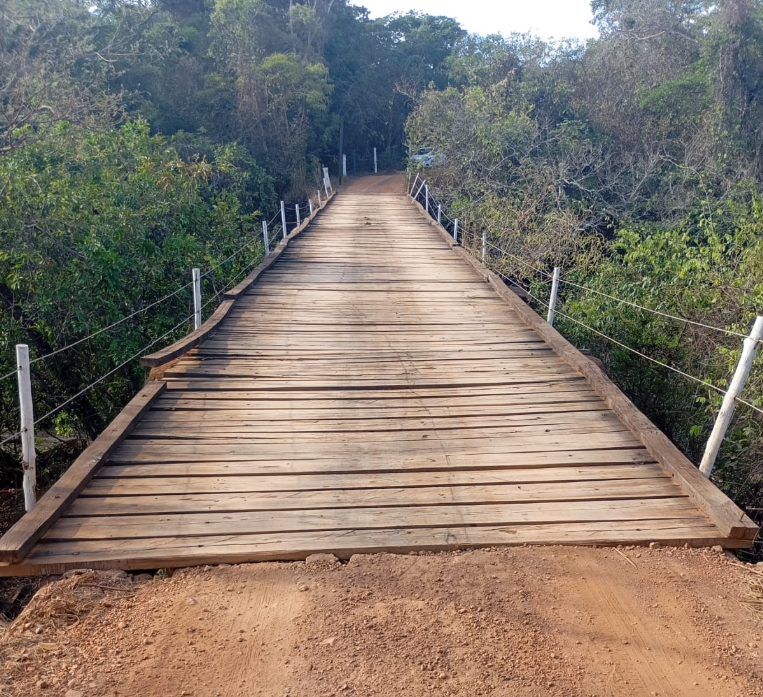
\includegraphics[width=\textwidth]{imgs/Rio do Braço.png}
        \caption{Ponte Rio do Braço}
        %\label{fig:ponte_a}
    \end{subfigure}
    %\hfill
    % \begin{subfigure}[t]{0.31\textwidth}
    %     \centering
    %     \includegraphics[width=\textwidth]{}
    %     \caption{Ponte R. Mascarenhas Morais}
    %     %\label{fig:ponte_b}
    % \end{subfigure}
    % \hfill
    \begin{subfigure}[t]{0.36\textwidth}
        \centering
        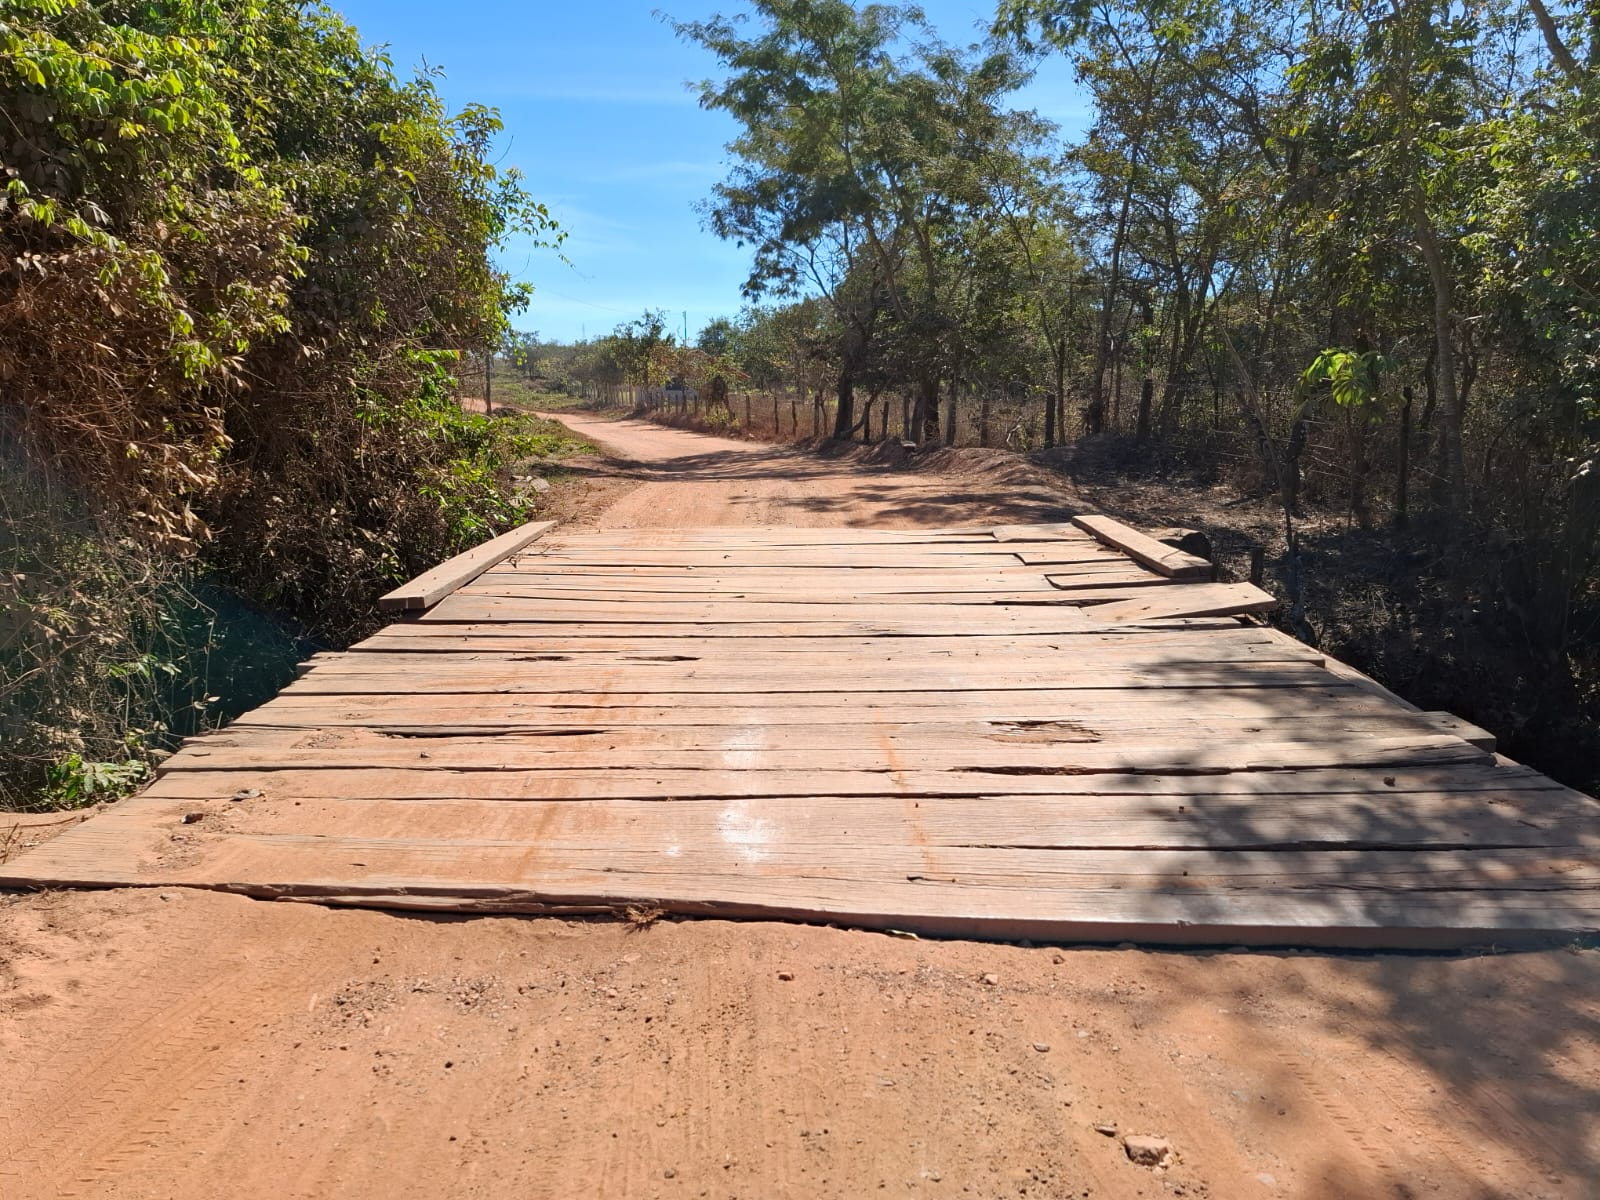
\includegraphics[width=\textwidth]{imgs/três bocas.jpg}
        \caption{Ponte Três Bocas}
        % \label{fig:ponte_c}
    \end{subfigure}
     % \legend{(a) Ponte Rio do Braço; (b) Ponte R. Mascarenhas Morais; (c) Ponte Três Bocas.}
\end{figure}

\begin{table}[htpb!]
\centering
\caption{Características das Pontes}
\label{tab_pontes}
\footnotesize
\begin{tabular}{
>{\centering\arraybackslash}m{1.8cm}
>{\centering\arraybackslash}m{1.5cm}
>{\centering\arraybackslash}m{1.5cm}
>{\centering\arraybackslash}m{2cm}
>{\centering\arraybackslash}m{1.5cm}
>{\centering\arraybackslash}m{2cm}
>{\centering\arraybackslash}m{2.5cm}
}
\hline
\textbf{Ponte} & \textbf{Comp.} & \textbf{Larg.} & \textbf{Madeira} & \textbf{Q. Long.} & \textbf{Dia. Long.} & \textbf{Pilares} \\ 
\hline
\multirow{2}{*}{Rio do Braço} & \multirow{2}{*}{42 m} & \multirow{2}{*}{3,50 m} & Eucalipto & \multirow{2}{*}{6} & \multirow{2}{*}{45--57} & \multirow{2}{*}{Pedra} \\
& & & Aroeira & & & \\ 
%\hline
\multirow{2}{*}{Três Bocas} & \multirow{2}{*}{6,40 m} & \multirow{2}{*}{3,50 m} & Aroeira & 3 & \multirow{2}{*}{43--54} & \multirow{2}{*}{Concreto} \\ 
& & & Angico & 6 & & \\
%\hline
% Ponte 03 & 7 m & 7 m & Aroeira & 6 & 44--53 & Pedra \\ 
\hline
\end{tabular}
\end{table}
   
    
Com base na configuração típica observada nessas estruturas, o sistema estrutural considerado consiste em um tabuleiro de madeira composto por pranchas longitudinais, apoiadas sobre vigas longitudinais circulares de madeira (longarinas), regularmente espaçadas. O tabuleiro está sujeito a ações permanentes (peso próprio) e ações variáveis associadas ao tráfego (carga móvel). As cargas atuantes no tabuleiro são transferidas para as longarinas de apoio e modeladas como carregamentos uniformemente distribuídos ao longo do vão. Uma representação esquemática do sistema estrutural é apresentada na Figura~\ref{fig:Ponte Frontal}.

\begin{figure}[h!]
    \centering
    \caption{Representação do sistema estrutural da ponte em madeira.}
    \label{fig:Ponte Frontal}
    \includegraphics[width=0.35\textwidth]{imgs/Ponte Frontal.png}\\   
    \vspace{0.2cm}
    \centering \small Fonte: Autoria própria, 2025.
\end{figure}








\subsection{Framework}
dsdspsmdsmpssdpsd46546466522

215551

\subsection{Dimensioanmento parámetrico}



% Para avaliação da confiabilidade e análise de custo foi adotado o problema de \textit{benchmark} descrito na Figura \ref{fig:toy1} que consiste em uma edificação hipotética em alvenaria estrutural composta por 7 paredes. A altura de cada pavimento é 2,80 m e também para efeito de cálculo fora considerado um carregamento de 10 pavimentos sobre as paredes do térreo apresentada na Figura \ref{fig:toy1}.

% \begin{figure}[htpb!]
% \centering
% 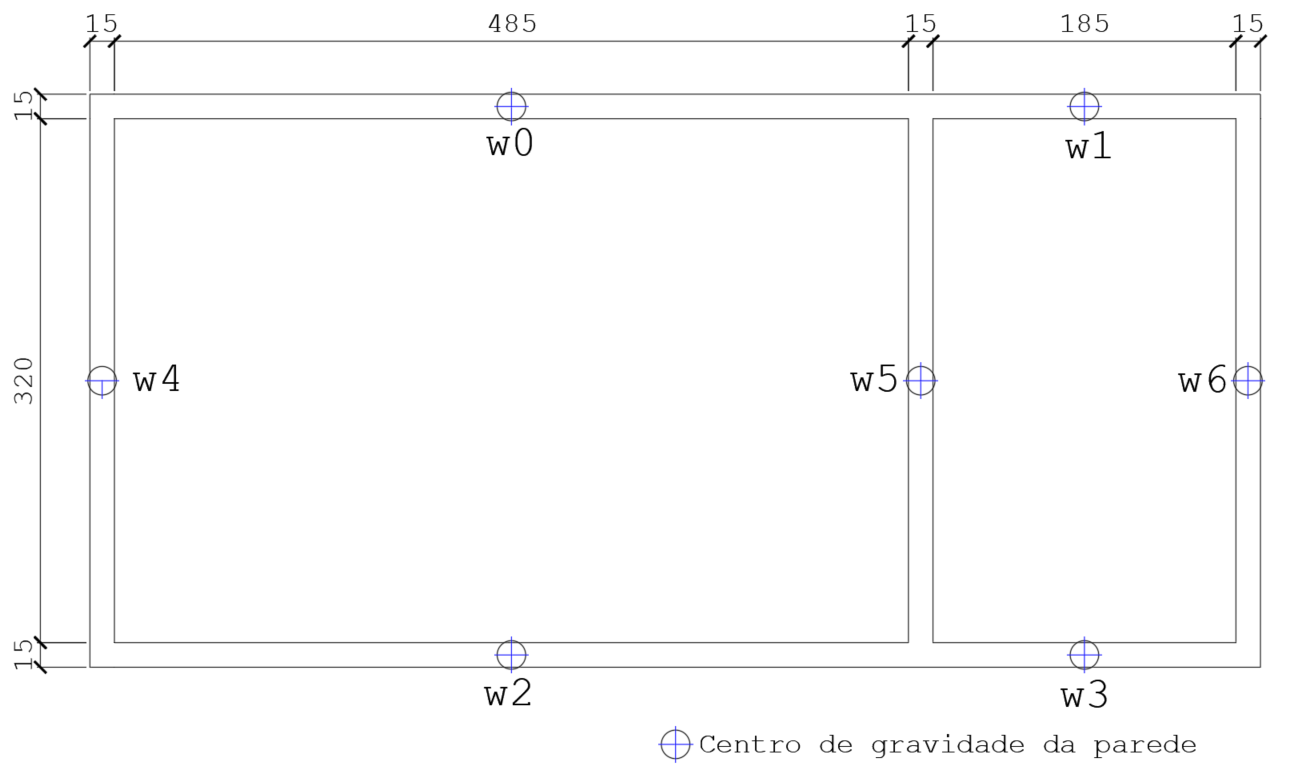
\includegraphics[width=0.9\textwidth]{imgs/benchmark1.png}
% \caption{Distribuição de paredes do edifício de alvenaria estrutural com dimensões em centímetros.}
% \label{fig:toy1}
% \end{figure}

% A Figura \ref{fig:toy2} apresenta os fatores de carregamento para o sistema intacto ($nlc$) e para a condição com remoção da parede $W_1$ ($r,w1$). No sistema sem remoção ($nlc$), o maior fator de carga é de 0,240, associado à parede $W_1$, indicando que esta é a mais solicitada na condição sem remoção de paredes. Já no sistema considerando a remoção da parede $W_1$ ($r,w1$), o maior fator de carga é de 0,285, referente à parede $W_5$. Esse aumento no fator de carregamento da parede $W_5$ decorre da redistribuição de esforços provocada pela remoção da parede $W_1$, resultando em um acréscimo na parcela de carga suportada pelas demais paredes.

% \begin{figure}[htpb!]
%     \centering
%     \begin{subfigure}[b]{0.48\textwidth}
%         \centering
%         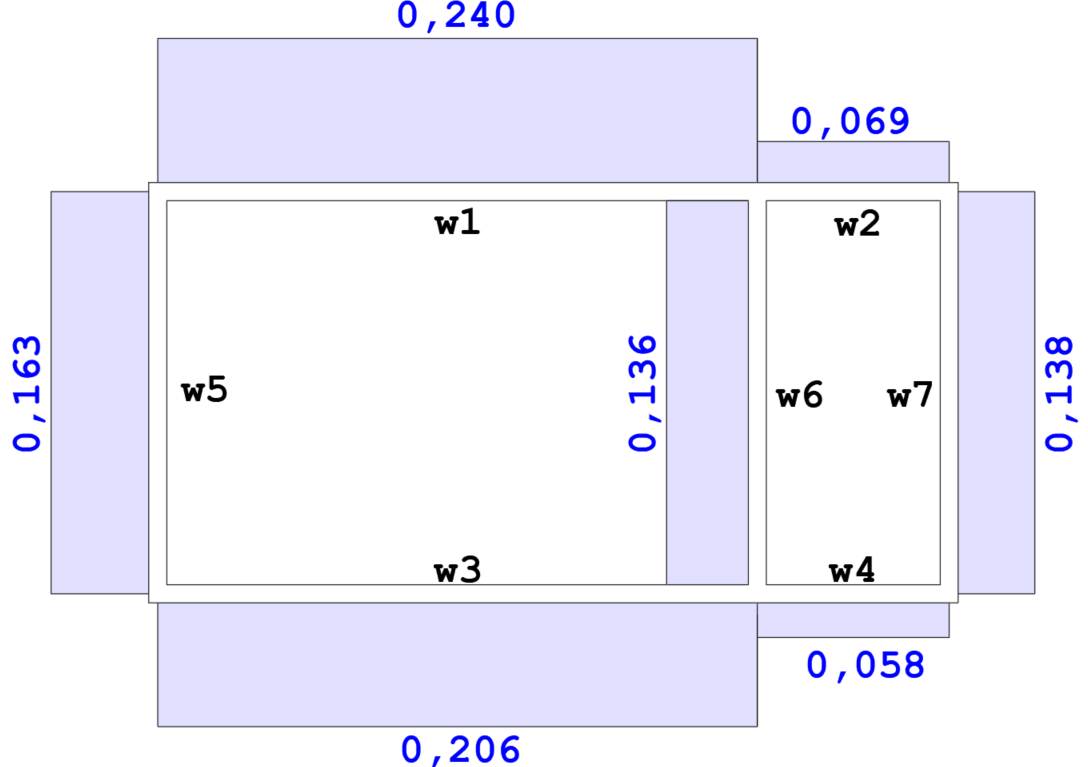
\includegraphics[width=\linewidth]{imgs/Sem remoção.png} % Substitua pelo seu arquivo
%         \caption{Sistema sem remoção de paredes}
%         \label{fig:toy2a}
%     \end{subfigure}
%     \hfill % Espaço entre as colunas
%     \begin{subfigure}[b]{0.48\textwidth}
%         \centering
%         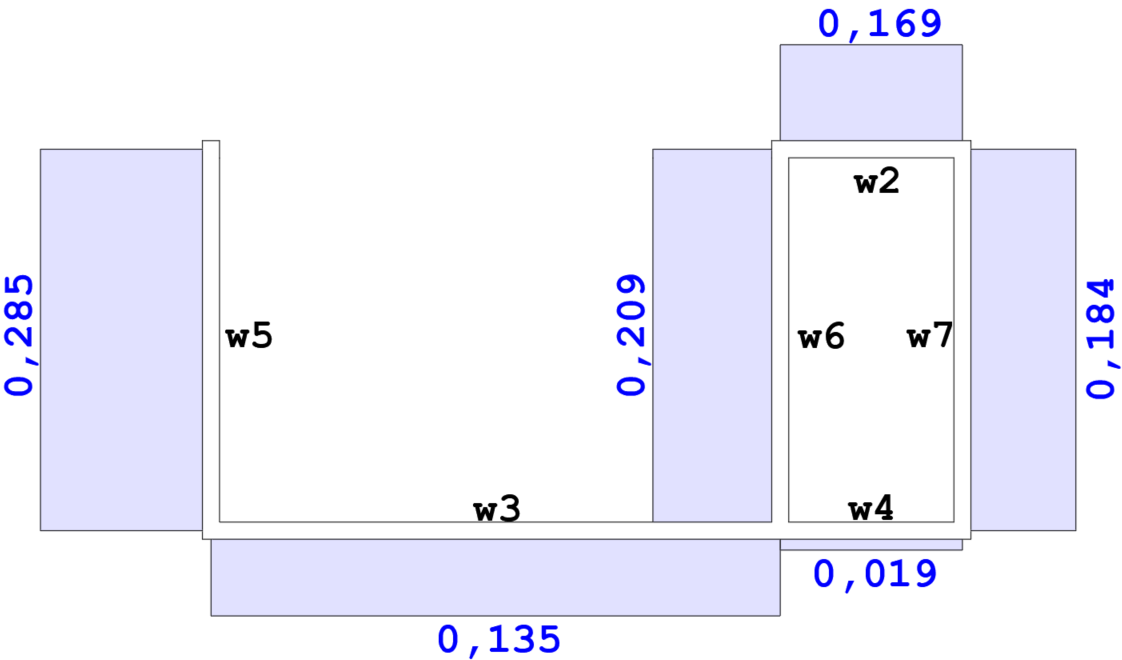
\includegraphics[width=\linewidth]{imgs/Com remoção.png} % Substitua pelo seu arquivo
%         \caption{Sistema com remoção da parede $W_1$}
%         \label{fig:toy2b}
%     \end{subfigure}
%     \caption{Fatores de esforço normal para sistema estrutural em paredes estruturais.}
%     \label{fig:toy2}
% \end{figure}

% Para a análise de confiabilidade do sistema estrutural foram adotadas as estatísticas apresentadas na Tabela \ref{tab:estatisticas}. No modelo considerado, $g$ representa o peso próprio da laje, enquanto $g_{ppl}$ corresponde à carga permanente adicional da laje, englobando revestimentos, argamassas e demais acabamentos fixos. O peso próprio das paredes é representado pela variável $g_{par}$.

% A carga variável de uso e ocupação da edificação para um período de referência de 50 anos é denotada por $q_k$, sendo adotado o valor de 1,50 kN/m², em conformidade com a ABNT NBR 6120. Para efeito de cálculo, foram considerados ainda os valores de 2,70 kN/m² para o peso próprio das paredes e 2,50 kN/m² para o peso próprio da laje. Já a carga $q_{apt}$ é a carga variável de uso e ocupação da edificação anual e será empregada na avaliação pós remoção da parede. A resistência característica do prisma de alvenaria ($f_{pk}$) representa o comportamento conjunto de blocos e argamassa. O fator de erro de resistência ($\theta_R$) expressa as incertezas relacionadas ao modelo de cálculo da resistência, enquanto o fator de erro de carregamento ($\theta_L$) representa as incertezas associadas à estimativa e modelagem das ações aplicadas.


% \begin{table}[htpb!]\footnotesize
% \centering
% \caption{Estatísticas das variáveis de projeto.}
% \label{tab:estatisticas}
% \begin{tabular}{c c c c c c}
% \toprule
% \textbf{Variável} & \textbf{Descrição} & \textbf{Média} & \textbf{CV} & \textbf{Distribuição} & \textbf{Referências} \\
% \midrule
% $g$ & Peso próprio da laje & $1,06 \cdot g$ & 0,12 & Normal & Santiago \textit{et al.} \cite{santiago_reliability-based_2020} \\
% $g_{ppl}$ & Carga permanente atuante nas lajes & $1,06 \cdot g_{ppl}$ & 0,12 & Normal & Santiago \textit{et al.} \cite{santiago_reliability-based_2020} \\
% $g_{par}$ & Carga permanente das paredes & $g_{par}$ & 0,02 & Normal & Isfeld \textit{et al.} \cite{isfeld_structural_2023} \\
% $q_{50}$ & Carga variável & $0,92 \cdot q_k$ & 0,25 & Gumbel máx. & Costa et al. \cite{costa_probabilistic_2022} \\
% $q_{apt}$ & Carga variável & $0,21 \cdot q_k$ & 0,76 & Gumbel máx. & Costa et al. \cite{costa_probabilistic_2022} \\
% $f_{pk}$ & Resistência característica do prisma & $1,36 \cdot f_{pk\text{}}$ & 0,24 & Normal & Santiago \textit{et al.} \cite{santiago_unreinforced_2024} \\
% $\theta_R$ & Erro de resistência & $0,95$ & 0,14 & Lognormal & Isfeld \textit{et al.} \ \cite{isfeld_structural_2023} \\
% $\theta_L$ & Erro de carga & $1$ & 0,05 & Lognormal & Costa et al. \cite{costa_probabilistic_2022} \\
% \bottomrule
% \end{tabular}
% \end{table}

% \subsection{Reinforced concrete versus Concrete Masonry: loss impact}

% A comparação entre estruturas de concreto armado e de alvenaria estrutural em cenários de perda de elementos revela diferenças marcantes no modo como os esforços se redistribuem. Na alvenaria estrutural, as cargas são predominantemente transmitidas por compressão axial e distribuídas ao longo das paredes. Essa configuração proporciona uma redistribuição mais homogênea, na qual a perda localizada de uma parede resulta em acréscimos de esforço relativamente modestos nos elementos adjacentes, como evidenciado na figura \ref{fig:toy2} desse artigo.

% Em contraste, nas estruturas de concreto armado compostas por vigas e pilares, a hiperestaticidade implica em redistribuições mais intensas. A retirada de um pilar ou apoio transfere esforços significativos para elementos vizinhos, gerando discrepâncias consideráveis em termos de flexão e esforço cortante. Embora a ductilidade do concreto armado e a formação de rótulas plásticas permitam ao sistema resistir temporariamente, o preço a pagar é a concentração elevada de esforços em pontos críticos, o que pode comprometer a durabilidade e acelerar o processo de degradação.

% \begin{figure}[htpb!]
% \centering
% 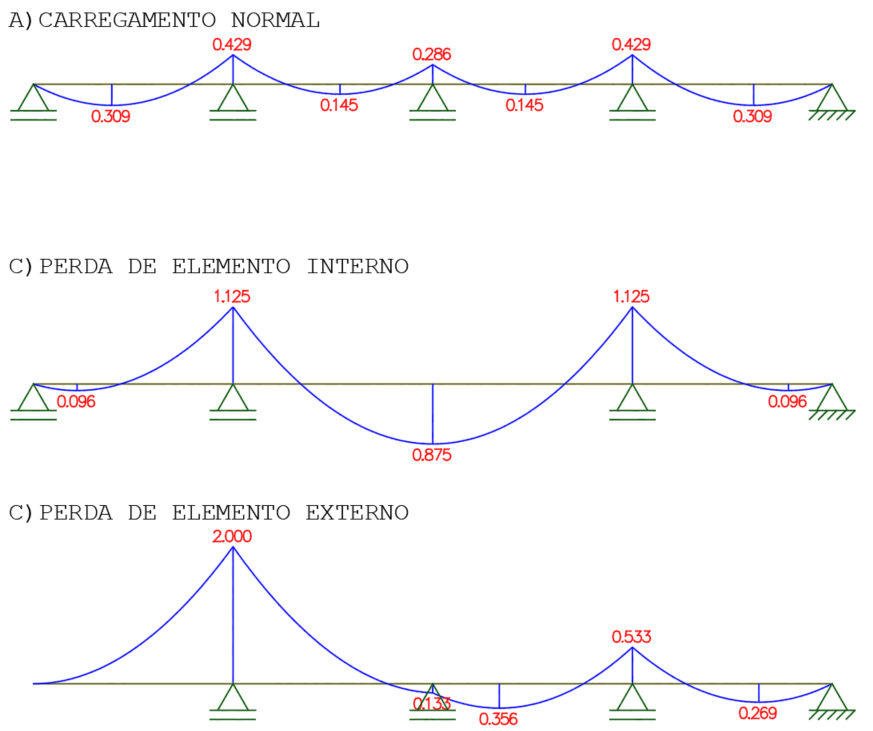
\includegraphics[width=0.8\textwidth]{imgs/intact_bean.png}
% \caption{Momentos fletores em viga contínua de quatro vãos: (a) Viga contínua intacta, todos os apoios presentes; (b) Redistribuição de esforços após remoção de um apoio central; (c) Redistribuição de esforços após remoção de um apoio lateral.}
% \label{fig:toy5}
% \end{figure}

% Os resultados obtidos em análises simplificadas no Ftool, com aplicação de carga unitária de 1 kN/m, ilustram esse contraste (figura \ref{fig:toy5}), enquanto nas paredes de alvenaria a variação de esforços normais se mantém em níveis relativamente uniformes após a perda de um elemento, em vigas e pilares de concreto armado surgem picos localizados de solicitação. Portanto, apesar da menor ductilidade, a alvenaria estrutural apresenta redistribuição mais equilibrada e previsível, minimizando as discrepâncias de esforços e reduzindo a vulnerabilidade a concentrações críticas em comparação às estruturas de concreto armado.

% \subsection{O projeto da edificação e avaliação da confiabilidade}

% A estrutura foi inicialmente projetada considerando a equações \eqref{eq:g_normal} e \eqref{eq:g_excepcional}. A Tabela \ref{tab:proj_alv1} apresenta os resultados para o valor de resistência de prisma necessária $\left(f_{pk}\right)$ para os carregamentos característicos indicados. Para a situação normal de carregamento e sem remoção de parede ($nlc$) foi avaliado o índice de confiabilidade da estrutura $\left(\beta_{nlc}\right)$. Após a remoção da parede estrutural $W1$ ($r,w1$) o índice de confiabilidade da estrutura $\left(\beta_{r,w1}\right)$ foi reavaliado. Na Tabela \ref{tab:proj_alv1} $g_{ppl}$ é calculado usando a equação \eqref{eq:gppl}.

% \begin{equation}
% g_{} = \frac{q_k}{L/D}
% \label{eq:gppl}
% \end{equation}

% \begin{table}[htpb!]
% \centering
% \caption{Resistências de prisma e índice de confiabilidade para o projeto estrutural em alvenaria considerando a equação \eqref{eq:g_normal}.}
% \label{tab:proj_alv1}
% \begin{tabular}{c c c c c c c}
% \toprule
% \textbf{L/D} & $g_{ppl} (MPa) $& $f_{bk}$ (MPa) & $f_{pk}$ (MPa)& $\beta_{nlc}$ & $\beta_{r,w1}$ & $\downarrow \Delta$ (\%)\\
% \midrule
% 1,00 & 1,50 & 6,00 & 4,50 & 2,59 & 1,99 & 23,4 \\
% 0,80 & 1,88 & 6,00 & 4,50 & 2,56 & 1,93 & 24,5 \\
% 0,60 & 2,50 & 6,00 & 4,50 & 2,51 & 1,85 & 26,5 \\
% 0,50 & 3,00 & 6,00 & 4,50 & 2,47 & 1,78 & 28,2 \\
% \bottomrule
% \end{tabular}
% \end{table}

% Observa-se que o índice de confiabilidade apresenta redução progressiva à medida que a carga permanente é elevada. Nos testes apresentados, essa redução foi, em média, da ordem de 25,65\%. Tal comportamento evidencia que o dimensionamento realizado conforme o método prescrito pela ASCE 7 \cite{american_society_of_civil_engineers_asce_asce_2013} pode conduzir a configurações estruturais associadas a probabilidades de falha relativamente elevadas, uma vez que valores de $\beta$ inferiores a 2,0 já se aproximam do limite de confiabilidade alvo geralmente aceito para elementos em regime de serviço. Nesse sentido, pode-se afirmar que os coeficientes parciais de segurança conservadores e o elevado grau de redundância característico das edificações em alvenaria estrutural tendem a mascarar os efeitos deletérios decorrentes da redistribuição de esforços após a remoção discricionária de uma ou mais paredes. Apesar disso é válido salientar que eventos de remoção discricionária de uma segunda parede são eventos com baixa probabilidade de ocorrência.

% \subsection{Análise de risco}

% Para analisar os efeitos da otimização de risco quando comparado ao método proposto pela ASCE 7 \cite{american_society_of_civil_engineers_asce_asce_2013} considera-se a proposta de Beck et al. \cite{beck_confiabilidade_2019} e Beck et al. \cite{beck_risk-based_2020} para construção da função objetivo conforme equação \eqref{eq:otm_risco}.

% \begin{equation}
% C_{ET}(\mathbf{\lambda_{pc}}) = C_C(\mathbf{\lambda_{pc}}) + C_{nlc} \cdot p_{c,nlc}(\mathbf{\lambda_{pc}}) + C_{ld} \cdot p_{c,ld}(\mathbf{\lambda_{pc}})
% \label{eq:otm_risco}
% \end{equation}

% Onde $C_{ET}$ é o custo total da edificação, $C_C$ o custo de construção da edificação. $C_{nlc}$ é o custo da falha total do sistema sob condições normais de carregamento. $C_{ld}$ é o custo da falha total do sistema dado um dano local prévio. $p_{c,nlc}$ e $p_{c,ld}$ são as probabilidades associadas aos eventos de colapso total da estrutura para condições normais de carregamento e um dano local, respectivamente. 

% As equações \eqref{eq:otm_risco_cc} a \eqref{eq:otm_risco_cld} representam os custos de construção e de falha. No caso os custos de falha são proporcionais ao custo de construção $C_C$.

% \begin{equation}
% C_C(\mathbf{\lambda_{pc}}) = \lambda_{pc}
% \label{eq:otm_risco_cc}
% \end{equation}

% \begin{equation}
% C_{nlc}(\mathbf{\lambda_{pc}}) = k \cdot \lambda_{pc}
% \label{eq:otm_risco_cnlc}
% \end{equation}

% \begin{equation}
% C_{ld}(\mathbf{\lambda_{pc}}) = k \cdot \lambda_{pc}
% \label{eq:otm_risco_cld}
% \end{equation}

% As equações \eqref{eq:otm_risco_pcnlc} e \eqref{eq:otm_risco_pcld} representam as probabilidades associadas aos eventos de falha on índices "NLC" corresponde a situação de condições normais de carregamento e "LD" a condição de dano local. Para este exemplo o dano local assumido consiste na remoção da parede $W_1$. 

% \begin{equation}
% p_{c,nlc}(\mathbf{\lambda_{PC}}) = P\left(C|NLC\right) \cdot P\left(NLC\right) 
% \label{eq:otm_risco_pcnlc}
% \end{equation}

% \begin{equation}
% p_{c,ld}(\mathbf{\lambda_{PC}}) = P\left(C|LD\right) \cdot P\left(LD\right) 
% \label{eq:otm_risco_pcld}
% \end{equation}

% Será considerado que a probabilidade de ocorrência do evento condições normais de carregamento ("NLC") é unitária e que a probabilidade de ocorrência de uma dano local varia entre $p_{ld}^{\min} \leq p_{ld} \leq 1$ onde $p_{ld}^{\min}$ é $5 \times 10^{-6}$ conforme Beck et al. \cite{beck_risk-based_2020}. As probabilidades $P\left(C|NLC\right)$ e $P\left(C|LD\right)$ são determinadas usando índice de Cornell conforme descrito na seção \ref{sec:confia}.

% Portanto o problema de otimização em minimizar o custo total da edificação em função de um custo de referência $\lambda_{pc}$, conforme equação \eqref{eq:otm_risco_min}. 

% \begin{equation}
% \begin{aligned}
% \text{Determinar } \lambda_{pc}^*, \\
% \text{minimizando} C_{TE}(\lambda_{pc}), \\
% \text{sujeito a: } \lambda_{pc} > 0.
% \end{aligned}
% \label{eq:otm_risco_min}
% \end{equation}


% \subsection{Arquitetura}
% O software é desenvolvido na linguagem Python, adotando uma arquitetura cliente-servidor. No lado do cliente, é disponibilizada uma interface web para entrada e visualização de dados, construída com a biblioteca Streamlit, o que resulta em uma interface simples, direta e intuitiva para o usuário. Já no lado do servidor, concentra-se todo o processamento computacional, englobando os cálculos estruturais determinísticos, como a verificação de tensões normais, flechas e esforços cortantes em elementos de madeira, bem como a análise probabilística, realizada por meio da implementação do método FORM (\textit{First-Order Reliability Method}) para a avaliação da confiabilidade estrutural.
% A escolha da linguagem Python deve-se, principalmente, ao seu amplo ecossistema de bibliotecas voltadas para análises numéricas e probabilísticas, além de sua ampla aceitação e utilização no meio acadêmico e científico, o que favorece a reprodutibilidade, a manutenção e a evolução do sistema.
% O fluxo de avaliação do gêmeo digital é organizado em três categorias principais de atividades: (a) o carregamento do cenário de análise desejado, no qual são definidos os dados geométricos, mecânicos e de carregamento da estrutura; (b) a escolha do nível de risco adotado, que estabelece os critérios de confiabilidade e segurança a serem considerados na avaliação; e (c) a aplicação do conceito de evidência e sua propagação em uma rede complexa, permitindo a integração das informações determinísticas e probabilísticas no processo de tomada de decisão. Cada uma dessas etapas é detalhada de forma a fornecer uma visão geral do funcionamento do gêmeo digital aplicado à análise do planejamento estrutural proposto.



% \subsection{Cenários de Upload de Conjunto de Dados e Método do Caminho Crítico}
% No contexto de cenários de upload de conjuntos de dados, o código foi estruturado para operar a partir de vetores de amostras que representam diferentes realizações possíveis das variáveis aleatórias do problema. Essas amostras podem ser interpretadas como cenários importados de um conjunto de dados externo, como planilhas ou bases de dados previamente preparadas. Cada linha do array \texttt{samples} corresponde a um cenário independente, contendo valores associados às cargas permanentes, cargas variáveis, resistências mecânicas e módulo de elasticidade. Esse formato é compatível com arquiteturas em que os dados são inicialmente organizados, validados e, posteriormente, carregados para processamento, de forma análoga ao upload de arquivos em aplicações interativas. A função \texttt{obj\_confia} concentra essa etapa, pois recebe todas as amostras simultaneamente e avalia, cenário a cenário, a função estado limite, retornando um vetor \texttt{g} que expressa a margem de segurança estrutural associada a cada realização.

% A consistência dos dados é garantida implicitamente pela própria estrutura do modelo. Assim como ocorre em sistemas de upload de cenários, nos quais colunas duplicadas, ausentes ou mal definidas inviabilizam a análise, cada posição do vetor de amostras possui um significado físico específico. Caso a ordem ou a quantidade de variáveis não seja respeitada, o modelo deixa de representar adequadamente o comportamento estrutural da viga. Dessa forma, a correta definição do \textit{dataset} é fundamental para que o método de confiabilidade forneça resultados fisicamente coerentes, como índices de confiabilidade $\beta$ e probabilidades de falha realistas.

% A parte determinística do código constitui a base da avaliação de cada cenário. Funções como \texttt{prop\_madeiras}, \texttt{momento\_max\_carga\_permanente}, \texttt{momento\_max\_carga\_variavel} e \\\texttt{coef\_impacto\_vertical} são responsáveis pelo cálculo das propriedades geométricas da seção e dos esforços internos a partir dos dados de entrada. Na sequência, são realizadas as verificações normativas de flexão, flecha e cisalhamento. Esse encadeamento de cálculos pode ser associado ao conceito de caminho crítico, no sentido de que existe uma sequência lógica obrigatória de etapas que deve ser respeitada para que a verificação estrutural seja válida. Caso alguma dessas etapas seja mal definida ou apresente inconsistências, todas as verificações subsequentes perdem seu significado físico.

% Dentro dessa lógica, a função \texttt{checagem\_longarina\_madeira\_flexao} pode ser interpretada como o caminho crítico do modelo estrutural. Ela reúne o cálculo dos esforços solicitantes, as combinações de ações, a aplicação do coeficiente de impacto vertical e, por fim, as verificações de estado limite. De forma análoga ao Método do Caminho Crítico no planejamento de projetos, em que o prazo total é governado pelas atividades críticas, a segurança global da longarina é governada pela condição mais desfavorável entre as verificações. O valor da função estado limite $g$ traduz exatamente esse ponto crítico, pois representa a diferença entre a resistência disponível e a solicitação atuante.

% Quando a análise probabilística é acionada, por meio da função \texttt{confia\_flexao\_pura}, o código passa a considerar explicitamente as incertezas associadas às variáveis de entrada. Para isso, são adotadas distribuições estatísticas, assumindo-se distribuições normais com coeficiente de variação de 10\%. O método FORM é então empregado para identificar o ponto mais provável de falha, que pode ser interpretado como o cenário crítico no espaço probabilístico. De maneira análoga ao conceito de caminho crítico em cronogramas, esse ponto domina o comportamento global do sistema, uma vez que pequenas variações em sua vizinhança provocam alterações significativas na probabilidade de falha.

% No que se refere à arquitetura da ferramenta, o \textit{dataset} da viga foi concebido para permitir três tipos distintos de dimensionamento: à flexão, à flecha e ao cisalhamento. Cada um desses modos de dimensionamento segue o mesmo fluxo lógico de avaliação determinística e, posteriormente, de análise de confiabilidade. A partir dessa estrutura, a ferramenta incorpora seis funcionalidades principais, combinando o dimensionamento da seção e a análise de confiabilidade para os três tipos de verificação. Essa abordagem integrada permite não apenas verificar se a viga atende aos critérios normativos em cada modo de solicitação, mas também quantificar o nível de confiabilidade associado a cada um deles, oferecendo uma visão mais completa e consistente do desempenho estrutural frente às incertezas dos carregamentos e das propriedades da madeira.


% \subsection{Análise de risco}
% ```latex
% O código implementa um modelo integrado para a análise estrutural de longarinas de madeira, avaliando os principais estados limites associados à flexão, à flecha e ao cisalhamento, com base nos fundamentos da Resistência dos Materiais e nos critérios normativos estabelecidos pela NBR~7190. A implementação é organizada em funções modulares e independentes, cada uma responsável por uma etapa específica do processo de cálculo. Essa estrutura garante consistência nos resultados, independentemente das combinações de carregamento e das propriedades dos materiais adotadas, além de facilitar o entendimento do fluxo lógico e físico que relaciona as ações externas às respostas estruturais da viga.

% Inicialmente, as propriedades geométricas da seção transversal são determinadas pela função \texttt{prop\_madeiras}. Para seções retangulares, a área, os momentos de inércia, os módulos de resistência e os raios de giração são obtidos diretamente a partir das dimensões de base e altura. Para seções circulares, essas grandezas são calculadas em função do diâmetro, utilizando as relações clássicas da geometria. Essas propriedades são fundamentais, pois estabelecem a ligação entre os esforços internos, como momentos fletores e esforços cortantes, e as tensões e deformações correspondentes desenvolvidas no material.

% Na sequência, o código calcula os esforços solicitantes decorrentes das cargas atuantes. O momento fletor máximo gerado pela carga permanente distribuída é determinado considerando uma viga biapoiada, segundo a expressão
% \[
% M = \frac{p\,l^{2}}{8},
% \]
% que representa a condição crítica no meio do vão. Para as cargas variáveis, o modelo incorpora um trem-tipo normativo, posicionado de forma a produzir o efeito mais desfavorável, combinando cargas concentradas, associadas às rodas, e cargas distribuídas, relacionadas à multidão. Adicionalmente, aplica-se um coeficiente de impacto vertical para representar os efeitos dinâmicos e vibratórios induzidos pelo tráfego, majorando os esforços de modo a simular uma condição de serviço mais realista.

% A verificação do estado limite último de flexão é realizada por meio da comparação entre a tensão normal solicitante e a resistência de cálculo da madeira. A tensão solicitante é obtida pela relação
% \[
% \sigma = \frac{M_d}{W},
% \]
% em que $M_d$ é o momento fletor de cálculo, resultante da combinação ponderada dos momentos característicos pelos coeficientes de segurança parciais, e $W$ é o módulo de resistência da seção. A resistência de cálculo da madeira é determinada a partir da resistência característica do material, multiplicada pelo coeficiente de modificação $k_{mod}$, que considera a duração do carregamento, a classe de umidade e o tipo de produto de madeira, e dividida pelo coeficiente de segurança do material $\gamma_w$. A condição de segurança é expressa por uma função estado limite que quantifica a diferença entre a capacidade resistente e a solicitação atuante.

% Paralelamente, é realizada a verificação do estado limite de serviço associado à flecha máxima da viga. A flecha é calculada com base na teoria da elasticidade, a partir de expressões deduzidas da equação diferencial da linha elástica, que relacionam o deslocamento ao carregamento, ao vão, ao módulo de elasticidade da madeira e ao momento de inércia da seção. O valor obtido é comparado com um limite normativo de deslocamento, geralmente definido como uma fração do vão, por exemplo, $l/360$. Essa verificação tem como objetivo garantir que as deformações permaneçam dentro de limites aceitáveis quanto ao conforto dos usuários, à funcionalidade da estrutura e à integridade dos elementos não estruturais.

% A resistência ao cisalhamento é avaliada por meio da determinação da tensão tangencial máxima na seção transversal. Para seções retangulares, considera-se a distribuição parabólica das tensões, resultando em uma tensão máxima igual a
% \[
% \tau = \frac{1{,}5\,V}{A},
% \]
% em que $V$ é o esforço cortante e $A$ é a área da seção. Para seções circulares, emprega-se uma formulação que envolve o esforço cortante, o momento estático, a largura da seção e o momento de inércia. A resistência de cálculo ao cisalhamento da madeira é usualmente estimada como uma fração da resistência à flexão, conforme indicado pela norma. A segurança é novamente avaliada por meio de uma função estado limite que contrapõe a resistência disponível à tensão solicitante de cálculo.

% Todas essas verificações são consolidadas em uma função principal, denominada \\\texttt{checagem\_longarina\_madeira\_flexao}, responsável por coordenar o fluxo completo da análise. Essa função organiza o cálculo dos esforços, a aplicação dos coeficientes de ponderação e de impacto e executa, de forma sequencial, as verificações de flexão, flecha e cisalhamento. De maneira análoga ao conceito de caminho crítico em análise de projetos, a segurança global do elemento é governada pelo estado limite mais desfavorável, uma vez que a falha em qualquer um desses modos compromete a integridade da viga.

% Por fim, o código extrapola a análise puramente determinística ao incorporar uma avaliação probabilística da confiabilidade estrutural por meio da função \texttt{confia\_flexao\_pura}. Nessa abordagem, as variáveis fundamentais de entrada, como cargas e resistências do material, são tratadas como variáveis aleatórias, descritas por distribuições de probabilidade. O método FORM (\textit{First-Order Reliability Method}) é então aplicado. Para cada realização das variáveis aleatórias, calcula-se o valor da função estado limite, e o algoritmo do FORM identifica iterativamente o ponto de projeto sobre a superfície de falha, estimando o índice de confiabilidade $\beta$. Dessa forma, o sistema não se restringe a uma resposta binária de atendimento ou não atendimento, mas fornece uma quantificação da probabilidade de falha da longarina, oferecendo uma avaliação mais realista da segurança estrutural ao considerar explicitamente as incertezas inerentes aos parâmetros de projeto.
% ```


% \subsection{Exemplo detalhado de verificação de uma longarina de madeira}

% Este exemplo ilustra o processo de dimensionamento de uma longarina de madeira com seção circular, submetida a uma combinação de ações permanentes e variáveis. O propósito da análise é verificar a segurança do elemento estrutural frente aos Estados Limites Últimos (ELU) e aos Estados Limites de Serviço (ELS), em conformidade com os critérios estabelecidos pela NBR 7190:2022.

% O procedimento é apresentado de forma detalhada, contemplando todas as etapas de cálculo essenciais ao atendimento dos requisitos normativos. Os dados iniciais englobam a geometria da viga, as características dos carregamentos atuantes, as propriedades mecânicas da madeira e os coeficientes de ponderação associados às ações e às resistências.

% Para o presente estudo, foram adotadas as variáveis de entrada descritas a seguir.

% \begin{table}[H]
% \centering
% \caption{Dados da viga de madeira}
% \begin{tabular}{ll}
% \hline
% \textbf{Parâmetro} & \textbf{Valor} \\ 
% \hline
% \multicolumn{2}{l}{\textbf{Geometria da viga}} \\
% Seção & Circular \\
% Diâmetro & $d = 0{,}49\;\text{m}$ \\
% Vão teórico & $L = 13{,}4\;\text{m}$ \\
% \hline
% \multicolumn{2}{l}{\textbf{Carregamentos atuantes}} \\
% Carga permanente distribuída & $p_{gk} = 1{,}7177\;\text{kN/m}$ \\
% Carga por roda (pontual) & $p_{\text{rodak}} = 40\;\text{kN}$ \\
% Carga de multidão & $p_{qk} = 4\;\text{kN/m}$ \\
% Distância entre eixos de rodas & $a = 1{,}5\;\text{m}$ \\
% \hline
% \multicolumn{2}{l}{\textbf{Propriedades da madeira}} \\
% Classe de carregamento & Permanente \\
% Classe da madeira & Natural \\
% Classe de umidade & 1 \\
% Resistência à compressão paralela & $f_{c0k} = 40{.}000\;\text{kN/m}^2$ \\
% Resistência à tração paralela & $f_{t0k} = 40{.}000\;\text{kN/m}^2$ \\
% Módulo de elasticidade & $E = 14{.}500{.}000\;\text{kN/m}^2$ \\
% \hline
% \multicolumn{2}{l}{\textbf{Coeficientes de segurança}} \\
% Ações permanentes & $\gamma_g = 1{,}3$ \\
% Ações variáveis & $\gamma_q = 1{,}5$ \\
% Resistência da madeira & $\gamma_{wc} = 1{,}4$ \\
% \hline
% \end{tabular}
% \end{table}

% Quando a peça de madeira apresenta variação de diâmetro ao longo do seu comprimento é necessário utilizar um diâmetro equivalente para representar a seção em cálculo. Esse valor, indicado para simplificar a análise, pode ser obtido a partir dos diâmetros mínimo e máximo da peça, segundo a expressão:

% \[
% d_{eq} = d_{\min} + \frac{d_{\max} - d_{\min}}{3}
%        = 44 + \frac{54 - 44}{3}
%        = 44 + \frac{10}{3}
%        = 47{,}33 \text{ cm}
% \]

% O uso do diâmetro equivalente garante que as propriedades geométricas, como área, momento de inércia e módulos resistentes, sejam avaliadas de forma mais realista, refletindo o comportamento de uma seção que não é constante ao longo do elemento.

% Sendo assim, o procedimento inicia-se pela determinação das propriedades geométricas da seção transversal circular, sendo essenciais para as verificações estruturais subsequentes.

% Para a viga com seção circular de diâmetro $d$, as propriedades geométricas são obtidas conforme as expressões a seguir.

% A área da seção é dada por:
% \[
% A = \frac{\pi d^2}{4}
%     = 0{,}1886\;\text{m}^2.
% \]

% Para seções circulares, os momentos de inércia em relação aos eixos principais são idênticos:
% \[
% I_x = I_y = \frac{\pi d^4}{64}
%         = 0{,}002836\;\text{m}^4.
% \]

% O módulo resistente também é o mesmo nos dois eixos devido à simetria da seção:
% \[
% W_x = W_y = \frac{I_x}{d/2}
%           = 0{,}01158\;\text{m}^3.
% \]

% O módulo estático da seção é dado por:
% \[
% S_x = S_y = A \cdot \frac{d}{2}
%           = 0{,}04621\;\text{m}^3.
% \]

% Os raios de giração nos dois eixos valem:
% \[
% r_x = r_y = \sqrt{\frac{I_x}{A}}
%           = 0{,}1227\;\text{m}.
% \]

% Para seções circulares, o coeficiente geométrico definido pela NBR~7190 é:
% \[
% k_m = 1{,}0.
% \]

% Essas propriedades caracterizam a rigidez e capacidade resistente da seção e serão usadas na verificação das tensões e flechas.

% Após a definição das propriedades geométricas, procede-se à determinação dos esforços solicitantes atuantes na longarina. Inicialmente, avalia-se o momento fletor decorrente da ação permanente distribuída ao longo do vão.

% No caso de cargas distribuídas uniformemente em vigas biapoiadas, o valor do momento fletor máximo é obtido pela expressão:

% \[
% M_{gk} = \frac{p_{gk} L^2}{8}
%        = 38{,}52\;\text{kN·m}
% \]

% Onde $M_{gk}$ é o momento fletor característico devido às ações permanentes \([\text{kN·m}]\), $p_{gk}$ representa a carga permanente distribuída ao longo da viga \([\text{kN/m}]\), e $L$ é o vão teórico do elemento estrutural \([\text{m}]\).

% Este valor representa o efeito exclusivamente da carga permanente própria da estrutura.

% Em seguida, procede-se à avaliação do momento fletor associado às ações variáveis. Para estruturas do tipo ponte, adota-se a modelagem correspondente ao trem-tipo especificado pela norma. No presente estudo, considerou-se uma ponte situada em estrada vicinal, para a qual a NBR 7190:2022 estabelece a utilização do modelo de carregamento TB-240.

% A ação variável é composta por duas parcelas:

% \begin{enumerate}
%     \item Cargas concentradas correspondentes às rodas do trem-tipo;
%     \item Carga distribuída adicional proveniente da ação de multidão.
% \end{enumerate}

% As rodas geram momento:
% \[
% M_{qk,\text{rodas}} 
% = \frac{3 p_{\text{rodak}} L}{4} - p_{\text{rodak}} a
% = 342\;\text{kN·m}
% \]

% Onde $l$ é o vão teórico da longarina, $p_{rodak}$ representa a carga variável característica aplicada por roda, e $p_{qk}$ corresponde à carga variável característica de multidão distribuída ao longo da peça. A variável $a$ define a distância entre os eixos das rodas consideradas na solicitação. O termo $m_{qk}$ representa o momento fletor máximo devido às ações variáveis, enquanto $c$ é o comprimento efetivo utilizado na ação distribuída adicional quando o vão ultrapassa $6\,\text{m}$.
% Como o vão é maior que $6\;$m, adiciona-se o efeito da carga de multidão. Primeiro, calcula-se o parâmetro geométrico:
% \[
% c = \frac{L - 4a}{2}
% = 3{,}7\;\text{m}.
% \]

% A contribuição da multidão:
% \[
% M_{qk,\text{multidão}} 
% = p_{qk}\frac{c^2}{2}
% = 27{,}38\;\text{kN·m}.
% \]

% O momento variável total antes do impacto:
% \[
% M_{qk} = 342 + 27{,}38 = 369{,}38\;\text{kN·m}.
% \]

% A norma exige aumento dinâmico para cargas móveis, por isso, aplica-se o coeficiente de impacto vertical:
% \[
% CIV = 1 + 1{,}06 \frac{20}{L + 50}
%      = 1{,}334.
% \]

% O momento amplificado é:
% \[
% M_{qk,\text{impacto}}
% = M_{qk} \left[ 1 + 0{,}75(CIV - 1) \right]
% = 461{,}91\;\text{kN·m}.
% \]

% A combinação última segue a NBR 8681:2025:

% \[
% M_{sd}
% = \gamma_g M_{gk} + \gamma_q M_{qk,\text{impacto}}
% = 742{,}95\;\text{kN·m}.
% \]

% O momento fletor resultante, obtido a partir das combinações de ações permanentes e variáveis, constitui o valor de referência para a verificação das tensões máximas no Estado Limite Último (ELU).  

% As expressões a seguir são utilizadas para determinar a flecha máxima da viga sob as ações permanentes e variáveis. A flecha devida à carga permanente é obtida pela formulação clássica para vigas biapoiadas com carregamento distribuído uniforme, enquanto a flecha causada pelas ações variáveis considera o efeito de cargas concentradas equivalentes às cargas transmitidas pelas rodas.

% \[
% \delta_{\max,g}
% =
% \frac{5 \cdot p_{gk} \cdot l^{4}}
% {384 \cdot E_{\text{med}} \cdot i_x}
% =
% 0{,}0176 \ \text{m}
% \]

% \[
% \delta_{\max,q}
% =
% \frac{p_{\text{rodak}}}
% {48 \cdot E_{\text{med}} \cdot i_x}
% \left[
% l^{3}
% +
% 2 \cdot \left(\frac{l - 2a}{2}\right)
% \cdot
% \left(
% 3l^{2}
% -
% 4 \cdot \left(\frac{l - 2a}{2}\right)^{2}
% \right)
% \right]
% =
% 0{,}1398 \ \text{m}
% \]

% Onde $\delta_{gk}$ é a flecha máxima causada pela carga permanente \([\text{m}]\), e $\delta_{qk}$ representa a flecha máxima causada pela carga variável \([\text{m}]\). O termo $p_{gk}$ é a carga permanente distribuída ao longo da viga \([\text{kN/m}]\), e $L$ é o vão teórico do elemento estrutural \([\text{m}]\). A variável $E$ corresponde ao módulo de elasticidade da madeira em flexão \([\text{kN/m}^2]\), e $I_x$ é o momento de inércia da seção transversal em relação ao eixo de flexão \([\text{m}^4]\). 

% A determinação das reações de apoio é necessária para a avaliação dos esforços solicitantes na viga. A reação devida à carga permanente é obtida diretamente da expressão clássica para vigas biapoiadas sob carregamento distribuído uniforme. Já a reação correspondente à carga variável considera a combinação de cargas concentradas por roda e, adicionalmente, a influência da carga distribuída referente à multidão.

% \[
% R_g
% =
% \frac{p_{gk} \cdot l}{2}
% =
% 11{,}5086 \ \text{kN}
% \]

% \[
% R_q
% =
% \frac{p_{\text{rodak}}}{l}
% \left(
% l + 3a + 2(l - 3a)
% \right)
% +
% \frac{p_{qk} \cdot (l - 3a)^2}{2 \cdot l}
% =
% 118{,}3896 \ \text{kN}
% \]

% Onde $R_{gk}$ é a reação de apoio devida à carga permanente \([\text{kN}]\) e $R_{qk}$ é a reação de apoio devida à carga variável \([\text{kN}]\). O termo $p_{gk}$ representa a carga permanente distribuída ao longo da viga \([\text{kN/m}]\), enquanto $L$ é o vão teórico da viga \([\text{m}]\). A variável $p_{rodak}$ corresponde à carga variável característica aplicada por roda \([\text{kN}]\), e $p_{qk}$ é a carga variável característica de multidão \([\text{kN/m}]\). A distância entre eixos das rodas é indicada por $a$ \([\text{m}]\). O termo auxiliar $d = L - 3a$ \([\text{m}]\) representa a posição relativa para consideração da parcela distribuída da ação variável no cálculo da reação.

% O cortante máximo na viga é determinado separando-se as contribuições das ações permanentes e das ações variáveis. Para a carga permanente distribuída, o valor de cortante segue diretamente da formulação clássica para vigas biapoiadas. Já o cortante máximo devido às ações variáveis considera o efeito conjunto das cargas por roda e da parcela distribuída correspondente à carga de multidão, de acordo com o esquema de carregamento adotado.

% \[
% v_g
% =
% \frac{p_{gk} \cdot l}{2}
% =
% 11{,}5086 \ \text{kN}
% \]

% \[
% v_q
% =
% \frac{p_{\text{rodak}}}{l}
% \left(
% 6a + 3(l - 3a - 2d)
% \right)
% +
% \frac{p_{qk} \cdot (l - 3a - 2h)^2}
% {2 \cdot l}
% =
% 107{,}1532 \ \text{kN}
% \]

% Onde $V_{gk}$ é o cortante máximo devido à carga permanente \([\text{kN}]\), enquanto $V_{qk}$ é o cortante máximo devido à carga variável \([\text{kN}]\). O termo $p_{gk}$ corresponde à carga permanente característica distribuída ao longo da viga \([\text{kN/m}]\) e $L$ é o vão teórico do elemento estrutural \([\text{m}]\). A variável $p_{rodak}$ representa a carga variável aplicada por roda \([\text{kN}]\), enquanto $p_{qk}$ é a carga variável característica de multidão \([\text{kN/m}]\). A distância entre os eixos das rodas é indicada por $a$ \([\text{m}]\) e $h$ representa a altura média da viga \([\text{m}]\). O parâmetro auxiliar $e = L - 3a - 2h$ \([\text{m}]\) define a posição efetiva considerada para a parcela distribuída da ação variável no cálculo do cortante.

% Concluída essa etapa, procede-se ao ajuste das resistências de cálculo da madeira por meio dos coeficientes de modificação.

% De acordo com o tipo de carregamento e com as condições ambientais às quais a estrutura estará submetida, adotam-se os coeficientes estabelecidos pela NBR 7190:2022, que permitem incorporar os efeitos da duração das ações e da classe de umidade na avaliação da resistência do material.

% \[
% k_{\text{mod1}} = 0{,}60 \qquad
% k_{\text{mod2}} = 1{,}00
% \]

% \[
% k_{\text{mod}} = k_{\text{mod1}} \times k_{\text{mod2}} 
%                = 0{,}60 \times 1{,}00 
%                = 0{,}60.
% \]


% Este coeficiente ajusta a resistência característica da madeira às condições reais de carregamento.

% Com os coeficientes de modificação definidos, procede-se ao cálculo das resistências de cálculo da madeira. As resistências de cálculo são determinadas a partir das resistências características da madeira, devidamente ajustadas pelos coeficientes normativos que representam os efeitos de modificação e os fatores parciais de segurança. Dessa forma, obtêm-se valores compatíveis com as condições de projeto e adequados às verificações no Estado Limite Último.

% \[
% f_{cd} 
% = \frac{f_{c0k}}{\gamma_{wc}} k_{\text{mod}}
% = 17{.}142{,}86\;\text{kN/m}^2.
% \]

% \[
% f_{td} 
% = \frac{f_{t0k}}{\gamma_{wc}} k_{\text{mod}}
% = 17{.}142{,}86\;\text{kN/m}^2.
% \]

% Como em flexão pura prevalece a menor das duas:
% \[
% f_{md} = \min(f_{cd}, f_{td})
% = 17{.}142{,}86\;\text{kN/m}^2.
% \]

% Concluídas as etapas de determinação dos esforços e das resistências de cálculo, efetuam-se as verificações pertinentes. Para a avaliação da tensão normal máxima, utiliza-se a seguinte relação:

% \[
% \sigma_x = \frac{M_{sd}}{W_x}
% = 64{.}159{,}76\;\text{kN/m}^2.
% \]

% A verificação das tensões normais na seção de madeira segue o critério de interação para estados limites últimos estabelecido pela NBR~7190. Para seções retangulares ou circulares, o modelo de verificação considera a combinação das tensões normais em ambos os eixos principais, ajustadas pelo coeficiente geométrico $k_m$. A formulação normativa é expressa pela condição:

% \[
% \frac{\sigma_x}{f_{md}} - k_m\,\frac{\sigma_y}{f_{md}} \leq 1
% \qquad \text{e} \qquad
% \frac{\sigma_y}{f_{md}} - k_m\,\frac{\sigma_x}{f_{md}} \leq 1.
% \]

% Essas inequações asseguram que a combinação das tensões paralelas aos eixos principais não ultrapasse a resistência de cálculo $f_{md}$, considerando o acoplamento entre as solicitações.

% Partindo da expressão normativa:

% \[
% \frac{\sigma_x}{f_{md}} - k_m\,\frac{\sigma_y}{f_{md}} \leq 1,
% \]

% multiplicando toda a inequação por $f_{md}$:

% \[
% \sigma_x - k_m \sigma_y \leq f_{md}.
% \]

% Reorganizando os termos:

% \[
% f_{md} - \sigma_x + k_m\,\sigma_y \ge 0.
% \]

% Chamando esta expressão de $g_1$:

% \[
% g_1 = f_{md} - \sigma_x + k_m\,\sigma_y.
% \]

% De forma análoga, para a segunda inequação normativa:

% \[
% \frac{\sigma_y}{f_{md}} - k_m\,\frac{\sigma_x}{f_{md}} \leq 1,
% \]

% multiplicando por $f_{md}$:

% \[
% \sigma_y - k_m \sigma_x \leq f_{md},
% \]

% reorganizando:

% \[
% f_{md} - \sigma_y + k_m\,\sigma_x \ge 0,
% \]

% definindo:

% \[
% g_2 = f_{md} - \sigma_y + k_m\,\sigma_x.
% \]

% Assim, a verificação final consiste em avaliar:

% \[
% g = \min(g_1,\, g_2)
% \]

% e a peça é considerada segura quando:

% \[
% g \ge 0.
% \]

% Esta forma é exatamente equivalente à formulação da NBR~7190, apenas rearranjada algébricamente para facilitar a implementação computacional.


% Onde $k_m$ é o coeficiente geométrico associado ao tipo de seção transversal (adimensional), $\sigma_x$ é a tensão normal atuante em relação ao eixo $x$ \([\text{kN/m}^2]\), e $\sigma_y$ é a tensão normal em relação ao eixo $y$ \([\text{kN/m}^2]\). A resistência de cálculo da madeira é denotada por $f_{md}$ \([\text{kN/m}^2]\). Os termos $g_1$ e $g_2$ representam as expressões de checagem derivadas das combinações de tensões exigidas pela norma, e $g = \max(g_1,g_2)$ é o valor final utilizado na análise. Quando $g \leq 1$, a seção atende ao estado limite último.

% Sendo assim, substituindo os valores do exemplo, resulta-se:

% \[
% f_{md} = 17{,}14 \text{ MPa}, \qquad
% k_m = 1{,}0, \qquad
% \sigma_x = 28{,}4918 \text{ MPa}, \qquad
% \sigma_y = 28{,}4918 \text{ MPa}.
% \]

% Cálculo de \( g_1 \)

% \[
% g_1 = f_{md} - \sigma_x + k_m \sigma_y
% \]

% Substituindo:

% \[
% g_1
% = 17{,}14 - 28{,}4918 + 1{,}0 \cdot 28{,}4918
% \]

% \[
% g_1 = 17{,}14
% \]

% Cálculo de \( g_2 \)

% \[
% g_2 = f_{md} - \sigma_y + k_m \sigma_x
% \]

% Substituindo:

% \[
% g_2
% = 17{,}14 - 28{,}4918 + 1{,}0 \cdot 28{,}4918
% \]

% \[
% g_2 = 17{,}14
% \]

% \subsection*{Valor final}

% \[
% g = \min(g_1,\, g_2) = 17{,}14
% \]

% \[
% g \ge 0 \quad \Rightarrow \quad \text{SEGURO}.
% \]

% A verificação da flecha da viga é realizada de acordo com os limites de deformação prescritos pela NBR~7190, os quais visam garantir o desempenho adequado do elemento estrutural em serviço. Para vigas submetidas a ações variáveis, o deslocamento vertical máximo deve ser comparado ao limite admissível estabelecido pela relação, sendo este o valor máximo permitido de flecha imediata.:

% \[
% \delta_{\mathrm{lim}} = \frac{L}{360},
% \]

% Substituindo:

% \[
% \delta_{\mathrm{lim}} = \frac{13{,}4}{360}
% \]

% \[
% \delta_{\mathrm{lim}} = 0{,}0372\ \text{m}
% \]

% A verificação do estado limite de deformações excessivas é então realizada pela inequação:

% \[
% g = \delta_{\mathrm{lim}} - \delta_{qk},
% \]

% Substituindo:

% \[
% g = 0{,}0372 - 0{,}025
% \]

% \[
% g = 0{,}0122\ \text{m}
% \]

% de modo que a viga atende ao critério de serviço sempre que:

% \[
% g \ge 0.
% \]

% Conclusão:

% \[
% g = 0{,}0122 \ge 0 \quad \Rightarrow \quad \text{SEGURO}.
% \]

% Onde $\delta_{\mathrm{lim}}$ é o limite de flecha admissível estabelecido pela norma \([\text{m}]\); $\delta_{qk}$ é a flecha máxima causada pela ação variável \([\text{m}]\); O valor $g$ expressa a equação do estado limite, e sua interpretação é direta: a deformação é considerada aceitável quando $g \ge 0$.

% A verificação da segurança ao cisalhamento em peças de madeira segue as recomendações da NBR 7190,
% consistindo na comparação entre a tensão de cisalhamento solicitante de cálculo e a resistência de
% cálculo da madeira ao cisalhamento paralelo às fibras.

% O esforço cortante de cálculo $V_{sd}$ resulta da combinação das ações permanentes e variáveis:

% \[
% V_{sd} = \gamma_g V_{gk} + \gamma_q V_{qk}
% \]

% onde:

% Onde $V_{gk}$ é o esforço cortante característico devido às ações permanentes \([\text{kN}]\); 
% $V_{qk}$ é o esforço cortante característico decorrente das ações variáveis \([\text{kN}]\); 
% $\gamma_g$ representa o coeficiente de ponderação aplicado às ações permanentes; 
% e $\gamma_q$ corresponde ao coeficiente de ponderação das ações variáveis.

% A expressão da tensão de cisalhamento depende do tipo de seção transversal:

% (a) Seção circular:

% \[
% \tau_d = \frac{V_{sd} \, S_x}{d \, I_x}
% \]

% Onde $S_x$ é o momento estático da seção em relação ao eixo neutro \([\text{m}^3]\); 
% $d$ corresponde ao diâmetro da seção transversal \([\text{m}]\); 
% e $I_x$ representa o momento de inércia da seção circular em relação ao eixo $x$ \([\text{m}^4]\).

% (b) Seção retangular:

% \[
% \tau_d = \frac{1.5 \, V_{sd}}{A}
% \]

% Onde $A$ é a área da seção transversal da viga \([\text{m}^2]\).

% A NBR 7190 define a resistência de cálculo ao cisalhamento paralelo às fibras como:

% \[
% f_{v0,d} = 0.10 \, f_{md}
% \]

% Onde $f_{md}$ é a resistência de cálculo da madeira à compressão paralela às fibras \([\text{kN/m}^2]\).

% A peça é considerada segura se a resistência for maior ou igual à solicitação:

% \[
% g = f_{v0,d} - \tau_d
% \]

% \[
% \text{Se } g \geq 0 \quad \Rightarrow \quad \text{OK}
% \]

% Assim, a verificação consiste em garantir que a tensão solicitante de cálculo não ultrapasse a
% resistência de cálculo ao cisalhamento.

% Do exemplo fornecido, têm-se:

% \[
% V_{sd} = 171{,}97\ \text{kN},
% \qquad
% \tau_d = 912{,}31\ \text{kN/m}^2,
% \qquad
% f_{v0,d} = 1714{,}29\ \text{kN/m}^2.
% \]

% \subsection*{Cálculo do estado limite}

% \[
% g = f_{v0,d} - \tau_d
% \]

% Substituindo:

% \[
% g = 1714{,}29 - 912{,}31
% \]

% \[
% g = 801{,}98\ \text{kN/m}^2
% \]

% \subsection*{Conclusão}

% \[
% g = 801{,}98 \ge 0 
% \quad \Rightarrow \quad \text{SEGURO}.
% \]

% \section{Análise de Confiabilidade Estrutural}

% A segurança probabilística da viga foi avaliada por meio do Método de Confiabilidade de Primeira Ordem (FORM),
% considerando como variáveis aleatórias:

% \[
% P_{gk},\; P_{rodak},\; P_{qk},\; f_{ck},\; f_{tk},\; E_{0,\mathrm{mean}}
% \]

% todas modeladas como distribuições normais com coeficiente de variação de 10\%:

% \[
% X_i \sim \mathcal{N}(X_{ik},\, 0.1\,X_{ik})
% \]

% A função de estado limite adotada foi:

% \[
% g(\mathbf{X}) = R(\mathbf{X}) - S(\mathbf{X})
% \]

% A falha ocorre quando:

% \[
% g(\mathbf{X}) < 0
% \]

% O FORM determina o ponto de falha mais provável e o índice de confiabilidade:

% \[
% \beta = \min_{\mathbf{u}} \| \mathbf{u} \| 
% \quad \text{sujeito a } g(\mathbf{u}) = 0
% \]

% A probabilidade de falha é calculada como:

% \[
% P_f = \Phi(-\beta)
% \]

% Aplicando o algoritmo usando o modelo da viga, obtiveram-se:

% \[
% \beta = 0.83, \qquad
% P_f = 0.203
% \]

% indicando probabilidade significativa de falha em relação ao estado limite de flexão.

% \subsection{Resumo dos Resultados}

% \begin{table}[H]
% \centering
% \begin{tabular}{lccc}
% \hline
% \textbf{Item} & \textbf{Obtido} & \textbf{Limite} & \textbf{Status} \\
% \hline
% Tensão de flexão & 3{,}74 & $\leq 1{,}0$ & Não atende \\
% Flecha máxima & $0{,}1395\;\text{m}$ & $0{,}0372\;\text{m}$ & Não atende \\
% Fator de utilização & 374\% & 100\% & Crítico \\
% Índice de confiabilidade $\beta$ & 0{,}83 & $\geq 3{,}0$ & Não atende \\
% Probabilidade de falha $P_f$ & 0{,}203 & $\leq 0{,}00135$ & Crítico \\
% \hline
% \end{tabular}
% \end{table}

% Os resultados indicam que a viga não atende às exigências de segurança nos critérios determinísticos
% nem probabilísticos.


% % --------------------------------------------------------------
% \section{Conclusão}

% Os resultados demonstram que a longarina de diâmetro $49\;\text{cm}$ não atende aos critérios da NBR 7190:1997. As tensões excedem o limite da espécie em aproximadamente 274\%, e a flecha ultrapassa o limite de serviço em 275\%. Assim, a peça encontra-se significativamente subdimensionada.

% Dessa forma é recomendado, aumentar o diâmetro da seção transversal, utilizar madeira com maior resistência estrutural, reduzir o vão da longarina ou adotar reforços estruturais ou sistemas mistos.



        \label{study_case}
\section{Concluding remarks}        \input{Section5.tex}        \label{concl}

\section{Agradecimentos}
\input{agradecimentos}




\bibliographystyle{model1-num-names}
\bibliography{mybibfile.bib}

\end{document}
